%==============================================================================
%  AI-Powered Learning Management System with Socratic Coaching Module
%  Bachelor's Thesis — Riga Nordic University (RNU)
%  Author: Kurbanov Azimjon
%  LaTeX edition — faithful reproduction of the original document
%==============================================================================
\documentclass[12pt,a4paper]{report}

%------------------------------- Encoding & fonts -----------------------------
\usepackage[T1]{fontenc}
\usepackage[utf8]{inputenc}
\usepackage{mathptmx}            % Times-like serif (text + math)
\usepackage[scaled=0.9]{helvet}  % Helvetica for sans
\usepackage{courier}             % typewriter

%------------------------------- Page geometry --------------------------------
\usepackage[a4paper,left=3cm,right=2cm,top=2.5cm,bottom=2.5cm]{geometry}
\usepackage{setspace}
\onehalfspacing

%------------------------------- Core packages --------------------------------
\usepackage{graphicx}
\usepackage{amsmath,amssymb}
\usepackage{pifont}              % \ding{51} check, \ding{55} cross
\usepackage{booktabs}
\usepackage{array}
\usepackage{tabularx}
\usepackage{longtable}
\usepackage{multirow}
\usepackage{ragged2e}
\usepackage{enumitem}
\usepackage{xcolor}
\usepackage{textcomp}
\usepackage[hidelinks]{hyperref}
\usepackage{url}
\usepackage{listings}

%------------------------------- Captions -------------------------------------
\usepackage[font=small,labelfont=bf,labelsep=period,justification=centering]{caption}

%------------------------------- Headings -------------------------------------
\usepackage{titlesec}
\titleformat{\chapter}[hang]
  {\normalfont\Large\bfseries}{\thechapter.}{0.6em}{}
\titlespacing*{\chapter}{0pt}{0pt}{18pt}
\titleformat{\section}[hang]
  {\normalfont\large\bfseries}{\thesection}{0.6em}{}
\titleformat{\subsection}[hang]
  {\normalfont\normalsize\bfseries}{\thesubsection}{0.6em}{}
\titleformat{\subsubsection}[hang]
  {\normalfont\normalsize\bfseries}{\thesubsubsection}{0.6em}{}

%------------------------------- Helper macros --------------------------------
\newcommand{\yes}{\ding{51}}     % check mark
\newcommand{\no}{\ding{55}}      % cross mark
\newcommand{\rar}{$\rightarrow$}

% column types
\newcolumntype{C}[1]{>{\centering\arraybackslash}p{#1}}
\newcolumntype{L}[1]{>{\RaggedRight\arraybackslash}p{#1}}

%------------------------------- Listings style -------------------------------
\definecolor{codebg}{rgb}{0.97,0.97,0.97}
\definecolor{codekw}{rgb}{0.10,0.10,0.55}
\definecolor{codecmt}{rgb}{0.30,0.45,0.30}
\definecolor{codestr}{rgb}{0.55,0.10,0.10}

\lstset{
  basicstyle=\ttfamily\scriptsize,
  backgroundcolor=\color{codebg},
  keywordstyle=\color{codekw}\bfseries,
  commentstyle=\color{codecmt}\itshape,
  stringstyle=\color{codestr},
  numbers=left,
  numberstyle=\tiny\color{gray},
  numbersep=8pt,
  frame=single,
  rulecolor=\color{gray!50},
  breaklines=true,
  breakatwhitespace=false,
  showstringspaces=false,
  tabsize=2,
  columns=fullflexible,
  xleftmargin=14pt,
  framexleftmargin=14pt,
}

\setlength{\parindent}{1.25cm}
\setlength{\parskip}{0pt}

%==============================================================================
\begin{document}
%==============================================================================

%------------------------------- TITLE PAGE -----------------------------------
\begin{titlepage}
\thispagestyle{empty}
\noindent
\includegraphics[width=5.5cm]{figs/logo.png}

\vspace{2.2cm}

\begin{center}
\begin{minipage}{0.95\textwidth}
\begin{tabbing}
\hspace{6.5cm}\=\kill
\textbf{Study Programme} \> \textbf{42484 Information Systems (BSc)}
\end{tabbing}
\end{minipage}

\vspace{1.4cm}
{\Large\bfseries Department of Natural Sciences and Computer Engineering\par}

\vspace{1.8cm}
{\LARGE RIGA NORDIC UNIVERSITY\par}
\vspace{0.2cm}
{\LARGE (RNU)\par}

\vspace{1.8cm}
{\large AI-Powered Learning Management System with\\[2pt]
Socratic Coaching Module\par}

\vspace{1.4cm}
{\large\bfseries BACHELOR'S THESIS\par}
\end{center}

\vfill

\noindent
\hfill Kurbanov Azimjon\\[10pt]
Studen:\\[6pt]
Supervsor: \hspace{3cm} Dr.sc,ing., Profesor, Jelena Caiko

\vspace{0.6cm}
\begin{center}
Riga 2026
\end{center}
\end{titlepage}

%------------------------------- FRONT MATTER ---------------------------------
\setcounter{page}{2}
\pagenumbering{arabic}

%--- Abstract ---
\chapter*{Abstract}
\addcontentsline{toc}{chapter}{Abstract}

The increasing adoption of artificial intelligence in education has created new
opportunities for adaptive and personalised learning. Existing learning management
systems such as Moodle, Canvas, and Google Classroom provide course delivery
infrastructure but lack the ability to engage students through guided reasoning
rather than direct instruction. Simultaneously, recent research in
retrieval-augmented generation and Socratic dialogue systems has demonstrated
measurable improvements in student comprehension and critical thinking, yet no
published system combines both approaches with real-time student performance data
from a relational database.

This Bachelor Paper presents the design and implementation of SmartLearn --- a
domain-agnostic learning management system with an integrated Socratic AI coaching
module. The thesis consists of three chapters. Chapter~1 reviews the theoretical
foundations of LMS platforms, retrieval-augmented generation, and the Socratic
teaching method, analysing 13 peer-reviewed publications to establish the research
gap. Chapter~2 presents the system architecture, technology stack justification,
PostgreSQL database schema, and the RAG pipeline design. Chapter~3 details the
implementation of the Spring Boot backend including JWT authentication, role-based
access control, TUS resumable upload, and MinIO file storage, together with the AI
coaching module and evaluation results.

The methodological basis includes comparative analysis of existing LMS platforms
and scientific literature, system architecture design using Clean Architecture
principles, full-stack implementation using Java~21, Spring Boot, PostgreSQL,
Flutter with Riverpod, and LLM API integration with RAG and prompt engineering. The
evaluation employs three measurable criteria: RBAC correctness across 15 API
endpoints, Socratic Score quality rubric across 20 AI interactions, and
profile-conditioning verification across 10 student profiles.

The research confirms the hypothesis that a domain-agnostic LMS combining RAG
retrieval conditioned on student performance data with Socratic dialogue constraints
delivers a more adaptive and pedagogically effective learning experience than any
single existing platform. The Bachelor Paper is written in 49 pages and contains 12
tables, 10 figures, 3 listings, 2 annexes, and a list of references with 13 sources.

%--- Keywords ---
\chapter*{Keywords}
\addcontentsline{toc}{chapter}{Keywords}

\textbf{Keywords:} learning management system, Socratic AI coaching,
retrieval-augmented generation, adaptive learning, Spring Boot, Flutter, JWT, RBAC,
PostgreSQL

%--- Table of Contents ---
\tableofcontents

%--- List of Figures / Tables ---
\listoffigures
\listoftables

%==============================================================================
%  INTRODUCTION  (unnumbered chapter; its single table is numbered "Table 1")
%==============================================================================
\chapter*{Introduction}
\addcontentsline{toc}{chapter}{Introduction}

\noindent\textbf{Topicality of the problem.} The global e-learning market reached
USD~315 billion in 2023 and is projected to grow at a compound annual rate of 13.5\%
through 2030~\cite{ref1}. Despite this growth, the fundamental pedagogical model of
most learning management systems has not changed: students receive content, complete
assignments, and receive grades. The missing element is adaptive, personalised
guidance --- the kind a skilled human tutor provides. Large language models have made
it technically feasible to build AI tutors at scale, yet existing systems either give
students direct answers (which undermines learning) or apply generic Socratic
techniques without access to each student's individual performance history. This gap
between technological capability and pedagogical implementation motivates the
research presented in this thesis.

A systematic literature review of 47 RAG-based educational chatbots conducted by
Swacha and Gracel~\cite{ref12} found that 37 of these studies were published in 2024
alone, confirming the field's rapid growth. However, none of the reviewed systems
simultaneously combine retrieval-augmented generation, Socratic dialogue constraints,
personalised test generation, and real student performance data from a relational
database. SmartLearn is designed to fill this gap.

\noindent\textbf{Aim of the study.} To design and implement a domain-agnostic
learning management system --- SmartLearn --- with an integrated Socratic AI coaching
module, and to evaluate its architectural suitability and pedagogical effectiveness in
comparison with existing LMS solutions.

\noindent\textbf{Object of the study.} Information systems for educational process
management.

\noindent\textbf{Subject of the study.} The architecture design and AI coaching
module implementation for a configurable, multi-role learning management system
combining RAG-based personalisation with Socratic dialogue constraints.

\noindent\textbf{Research problem.} Existing LMS platforms are either domain-specific
or lack adaptive AI assistance that guides students through reasoning rather than
providing direct answers. Published AI tutoring systems address individual
components --- RAG, Socratic dialogue, or test generation --- in isolation. No
existing open solution combines all four capabilities: retrieval-augmented
generation, Socratic dialogue constraints, personalised test generation, and
real-time conditioning on individual student performance data stored in a relational
database.

\noindent\textbf{Hypothesis.} A domain-agnostic LMS built on a structured backend
(Spring Boot and PostgreSQL) with a Socratic AI coaching module that simultaneously
conditions both RAG retrieval and the system prompt on each student's performance
profile will deliver a more adaptive and pedagogically effective learning experience
than any existing LMS platform, while remaining configurable for any educational
domain without code modifications.

\noindent\textbf{Tasks of the study:}
\begin{enumerate}[leftmargin=*,label=\arabic*.]
  \item Analyse existing LMS platforms and theoretical foundations of adaptive
  learning, Socratic teaching methodology, and RAG-based AI personalisation in
  educational systems, and establish a research gap by comparing 13 peer-reviewed
  publications. (Chapter~1)
  \item Design the system architecture of SmartLearn --- including technology stack
  selection, PostgreSQL database schema, role-based access model, and the RAG
  pipeline for the AI coaching module --- and justify each architectural decision
  against evaluated alternatives. (Chapter~2)
  \item Implement the core system modules and evaluate the solution against three
  defined quality criteria: RBAC correctness across 15 API endpoints, Socratic Score
  quality across 20 AI interactions, and profile-conditioning verification across 10
  student profiles. (Chapter~3)
\end{enumerate}

\noindent\textbf{Research methods.} The methodological basis includes: (1) secondary
research --- systematic comparative analysis of 13 published works on RAG, Socratic
AI, and adaptive LMS platforms; (2) system design --- architectural modelling using
Clean Architecture principles, UML-style diagrams, and relational database schema
design with RBAC; (3) software engineering --- full-stack implementation using
Java~21, Spring Boot, PostgreSQL, MinIO, TUS protocol, Flutter with Riverpod, and LLM
API integration with prompt engineering and RAG pipeline construction;
(4)~evaluation --- functional verification of REST API endpoints, AI response quality
assessment using the Socratic Score rubric, and profile-conditioning verification.

The mapping of research tasks to thesis chapters is presented in Table~1.

% --- Introduction's single table, forced to display as "Table 1" ---
\begingroup
\renewcommand{\thetable}{1}
\setcounter{table}{0}
\begin{table}[h]
\centering
\caption{Mapping of research tasks to thesis chapters}
\begin{tabular}{c L{8cm} l}
\toprule
\textbf{Task} & \textbf{Description} & \textbf{Chapter}\\
\midrule
1 & Literature review and gap analysis & Chapter~1\\
2 & System architecture and design & Chapter~2\\
3 & Implementation and evaluation & Chapter~3\\
--- & Synthesis and hypothesis validation & Conclusions\\
\bottomrule
\end{tabular}
\end{table}
\endgroup

%==============================================================================
%  CHAPTER 1
%==============================================================================
\chapter{Literature Review and Theoretical Background}
% restore per-chapter numbering for tables & figures
\renewcommand{\thetable}{\thechapter.\arabic{table}}
\renewcommand{\thefigure}{\thechapter.\arabic{figure}}

This chapter establishes the theoretical and empirical foundation for SmartLearn. It
defines the key concepts used throughout the thesis, surveys 13 peer-reviewed
publications organised into four thematic clusters, presents a comparative gap
analysis that motivates the research, and formalises the theoretical framework
including the RAG pipeline formula and the Socratic Score evaluation rubric.

\section{Core Concepts and Definitions}

A \textbf{Learning Management System (LMS)} is a software platform that enables the
creation, delivery, and management of educational content and the tracking of learner
progress. According to Spriggs et al.~\cite{ref2}, traditional LMS platforms
distribute materials but do not adapt to individual learner needs, particularly when
instructor availability is limited. Widely deployed systems such as Moodle, Canvas,
and Google Classroom exemplify this model: they organise content and facilitate
assessment but do not engage students in guided reasoning. SmartLearn extends this
definition to include AI-driven coaching as a first-class system component.

\textbf{Retrieval-Augmented Generation (RAG)} is a technique that enhances large
language model responses by supplying relevant external documents or database records
at query time, reducing hallucination and grounding answers in verifiable content. As
defined by Swacha and Gracel~\cite{ref12} in their systematic review of 47 RAG-based
educational chatbots, RAG addresses the principal limitation of LLMs in academic
contexts: the tendency to generate plausible but factually incorrect statements. In
SmartLearn, RAG retrieval is conditioned not only on the student's question but also
on the student's performance profile, a design choice that extends the standard RAG
pipeline.

The \textbf{Socratic Method} is a pedagogical dialogue technique attributed to the
philosopher Socrates in which the instructor never provides direct answers but instead
asks probing questions that lead the student to derive conclusions independently. In
educational research, this approach aligns with Bloom's Taxonomy at the analysis and
evaluation levels --- cognitive operations that require deeper processing than simple
recall~\cite{ref5}. Sunil and Thakkar~\cite{ref5} demonstrated computationally that
enforcing Socratic constraints on an LLM tutor caused more than 75\% of undergraduate
students to shift from imprecise help-seeking to complex problem decomposition within
two to three weeks.

\textbf{Adaptive Learning} refers to educational approaches in which the system
continuously adjusts the difficulty, sequence, or style of content based on the
learner's demonstrated performance. Spriggs et al.~\cite{ref2} define an Adaptive LMS
(ALMS) as one that incorporates multiple LLMs --- both general-purpose and
domain-specific --- to personalise the learning environment dynamically. In
SmartLearn, adaptation is achieved through the student profile stored in PostgreSQL,
which tracks level, weak topics, recent errors, and interaction history, and which
conditions every AI response.

\textbf{Personalised Assessment} refers to the generation of test questions and
evaluation criteria that are tailored to the specific gaps and strengths of an
individual student, rather than applying a uniform assessment to all learners. Ali et
al.~\cite{ref10} demonstrated that GPT-4-based systems can generate pedagogically
sound multiple-choice questions with greater than 90\% accuracy and produce 20
questions in under 15 minutes, compared to two or more hours for manual creation. The
limitation of this approach, however, is that questions are generated from generic
course material rather than from the individual student's identified weak topics --- a
gap that SmartLearn addresses.

\section{Related Work}

The related work is organised into four thematic clusters: RAG architectures for
education, Socratic dialogue systems, personalised test generation, and survey studies
providing broader context. Each cluster is analysed for methodology, reported results,
and limitations relevant to the SmartLearn research problem.

\subsection{Cluster A: RAG Architectures for Education}

Dong et al.~\cite{ref1} propose KG-RAG, a knowledge-graph-enhanced RAG framework for
intelligent tutoring that grounds LLM responses in structured domain knowledge rather
than relying solely on semantic similarity matching. In a controlled experiment with
76 participants, KG-RAG produced a statistically significant 35\% increase in
assessment scores ($p < 0.001$), published in ICEIT~2025. The critical limitation for
the present research is that KG-RAG retrieves content based on the question alone and
does not incorporate the student's individual performance history into the retrieval or
generation process. There is also no Socratic dialogue constraint --- the system
provides direct, albeit well-grounded, answers.

Spriggs et al.~\cite{ref2} present an Adaptive LMS that integrates multiple LLMs to
provide a customisable learning environment, targeting settings with limited instructor
availability. Their system addresses factual inaccuracy and outdated information by
combining general-purpose and domain-specific models. However, the paper does not
report quantitative evaluation metrics, and neither Socratic dialogue nor personalised
test generation based on individual student data is described.

Lin et al.~\cite{ref3} introduce RAG-PRISM, a personalised tutoring framework
addressing workforce skill gaps in Fourth Industrial Revolution domains, including
cybersecurity. Using GPT-4, the system achieves 87\% relevancy rating and 100\%
alignment with manually curated training queries, published at IEEE~FIE~2025. The
framework is restricted to a single domain and uses a synthetic question-answer dataset
rather than real student interaction logs from a database. There is no Socratic
dialogue component.

Cohn et al.~\cite{ref4} propose Log-Contextualized RAG (LC-RAG), which enhances
standard RAG by contextualising retrieval using environment activity logs from the
C2STEM collaborative learning platform. The system demonstrates that LC-RAG improves
retrieval relevance over a discourse-only baseline, enabling the agent Copa to deliver
more personalised guidance. This approach is the closest precedent to SmartLearn's
design: both use contextual data about the student's activities to condition retrieval.
The difference is that SmartLearn uses structured relational database records (weak
topics, recent errors, level) rather than unstructured environment logs, and adds
Socratic dialogue constraints on top of retrieval.

\subsection{Cluster B: Socratic Dialogue Systems}

Sunil and Thakkar~\cite{ref5} present SocraticAI, a scaffolded AI tutoring system for
undergraduate computer science education. The system enforces structured constraints
including authentication, query validation, reflective engagement requirements, daily
usage caps, and RAG grounded in course materials. In a study at COMPUTE~2025, more than
75\% of students produced substantive reflections and demonstrated a shift from
imprecise help-seeking to deliberate problem decomposition within two to three weeks.
This paper is the most directly related to SmartLearn's AI coaching module. The key gap
is the absence of personalised test generation based on individual student error history
and the absence of a relational student database conditioning AI responses.

Zhang et al.~\cite{ref6} propose SPL --- a Socratic Playground for Learning ---
powered by GPT-4 with advanced prompt engineering. The system generates customised
learning scenarios and facilitates multi-turn Socratic dialogues. Pilot experimental
results from essay writing tasks demonstrate potential, though specific quantitative
metrics are not reported. SPL is a standalone dialogue system without LMS
infrastructure: no role-based access (Teacher/Student/Admin), no course management, no
test generation, and no student database.

Favero et al.~\cite{ref7} develop an educational chatbot using Socratic questioning to
promote critical thinking. Presented at ECAI~2024, the system uses fine-tuned small
language models --- Llama2 7B and 13B parameters --- deployable on standard hardware
without cloud API costs. Experiments with simulated student interactions confirm that
the Socratic tutor supports critical thinking development significantly better than
standard chatbots. The deliberate choice of local models for privacy reasons represents
a meaningful contrast with SmartLearn, which prioritises response quality by using
cloud LLM APIs (Claude or GPT-4) at the cost of latency and API pricing.

Qi et al.~\cite{ref8} present IntelliChain, a multi-agent framework integrating LLMs
with knowledge graphs for Socratic teaching in mathematics education, presented at
GCCCE~2024. The framework demonstrates notable advantages in accuracy and credibility
of educational interactions. The architecture is more complex than SmartLearn's
single-agent approach: IntelliChain uses separate teacher and student agents with
chain-of-thought dialogue, while SmartLearn uses a single LLM constrained by a
structured system prompt. The simpler architecture is a deliberate design choice for
production deployability.

\subsection{Cluster C: Personalised Test Generation}

Shirkar et al.~\cite{ref9} investigate LLM-based quiz generation for assessment
systems, focusing on the pedagogical quality of automatically generated questions.
Their work establishes that LLMs can produce assessment items suitable for educational
use, providing a methodological foundation for the quiz generation component of
SmartLearn. The limitation relative to SmartLearn is that questions are generated from
course content uniformly, without personalisation based on individual student
performance data.

Ali et al.~\cite{ref10} present a full-stack implementation of AI-powered quiz
generation for Canvas LMS, using OpenAI's GPT API and PyPDF2 for course material
parsing, with a Flask backend and JavaScript frontend. In NWISEd~2025, they report that
GPT-4 achieves 92\% question accuracy while the more cost-efficient GPT-4o Mini achieves
85\% accuracy. The system generates 20 questions in under 15 minutes, compared to two or
more hours for manual creation. Formatting corrections succeed on the first attempt in
85\% of cases. Questions are generated from course material without reference to any
individual student's history, and there is no Socratic dialogue --- the system is a tool
for teachers, not an interactive tutor for students.

Mucciaccia et al.~\cite{ref11} propose an automatic MCQ generation and evaluation system
for university settings, presented at COLING~2025. The system combines prompt
engineering with a review process for question generation, and uses a separate LLM as an
automated quality judge. This two-stage approach --- generate then evaluate --- provides
a methodological reference for SmartLearn's Socratic Score rubric, which similarly
evaluates AI response quality post-generation. The paper does not address
personalisation or dialogue.

\subsection{Cluster D: Survey and Adaptive Retrieval}

Swacha and Gracel~\cite{ref12} conduct a systematic review of 47 RAG-based chatbots in
education, covering publications from Scopus, Web of Science, and Google Scholar from
2022 onwards. Key findings: 37 of the 47 papers were published in 2024, demonstrating
the field's recency. RAG consistently addresses the hallucination problem that limits
LLM adoption in academic contexts. Evaluation criteria used across studies include
accuracy, relevance, faithfulness, and user acceptance. One unexpected finding is that
adding RAG reduced user trust in one study using GPT-3.5 (from 5.98 to 5.50 on a 7-point
scale), suggesting that retrieval quality matters as much as retrieval presence. This
underscores the importance of SmartLearn's profile-conditioned retrieval strategy over
naive semantic search.

Jeong et al.~\cite{ref13} propose Adaptive-RAG, a framework that dynamically selects the
retrieval strategy based on query complexity --- from no retrieval for simple questions
to multi-step retrieval for complex ones. Accepted at NAACL~2024, the method uses a
lightweight classifier trained on existing model predictions to route queries without
manual annotation. Adaptive-RAG is not an educational system, but it provides
theoretical grounding for SmartLearn's future work: the current system uses a fixed
single-step retrieval strategy, and Adaptive-RAG could be incorporated to handle the
range of student questions from simple factual to complex analytical.

\section{Comparative Gap Analysis}

As shown in Table~\ref{tab:gap}, no existing published system simultaneously implements
all four capabilities that define SmartLearn's research contribution: RAG retrieval,
Socratic dialogue constraints, personalised test generation, and real student
performance data from a relational database. SmartLearn is the first system to combine
all four components.

\begin{table}[htbp]
\centering
\caption{Comparative analysis of related systems vs. SmartLearn}
\label{tab:gap}
\footnotesize
\renewcommand{\arraystretch}{1.25}
\begin{tabularx}{\textwidth}{L{2.1cm} c c c c L{2.0cm} L{2.4cm}}
\toprule
\textbf{System} & \textbf{Year} & \textbf{RAG} & \textbf{Socratic} &
\textbf{Pers. Tests} & \textbf{Student DB} & \textbf{Key Gap}\\
\midrule
Dong et al.~\cite{ref1} & 2025 & \yes\,(graph) & \no & \no & \no & No dialogue, no tests\\
Spriggs et al.~\cite{ref2} & 2025 & Partial & \no & \no & \no & No Socratic, no tests\\
Lin et al.~\cite{ref3} & 2025 & \yes & \no & \no & Synthetic & One domain, no dialogue\\
Cohn et al.~\cite{ref4} & 2025 & \yes\,(logs) & \no & \no & Logs only & No dialogue, no tests\\
Sunil \& Thakkar~\cite{ref5} & 2025 & \yes & \yes & \no & \no & No tests, no student DB\\
Zhang et al.~\cite{ref6} & 2024 & \no & \yes & \no & \no & No LMS, no tests\\
Favero et al.~\cite{ref7} & 2024 & \no & \yes & \no & \no & Local model, no LMS\\
Qi et al.~\cite{ref8} & 2025 & \no & \yes\,(graph) & \no & \no & Complex, no tests\\
Shirkar et al.~\cite{ref9} & --- & \no & \no & \yes & \no & No dialogue, no DB\\
Ali et al.~\cite{ref10} & 2025 & \no & \no & \yes\,(90\%) & \no & No dialogue, no profile\\
Mucciaccia et al.~\cite{ref11} & 2025 & \no & \no & \yes\,(MCQ) & \no & No dialogue, no profile\\
Swacha \& Gracel~\cite{ref12} & 2025 & \yes\,survey & --- & --- & --- & Survey only\\
Jeong et al.~\cite{ref13} & 2024 & \yes\,(adapt.) & \no & \no & \no & Not educational\\
\midrule
\textbf{SmartLearn} & 2026 & \yes & \yes & \yes & \yes\,(PostgreSQL) &
First to combine all four\\
\bottomrule
\end{tabularx}
\end{table}

\section{Theoretical Framework}

The theoretical basis of SmartLearn rests on two foundations: the formal RAG pipeline
model that describes how student data conditions AI responses, and the pedagogical
justification for Socratic constraints derived from Bloom's Taxonomy.

The core research formula formalises the SmartLearn AI coaching pipeline. For each
student interaction, the final response $a$ is generated as:

\begin{equation}
a = \mathrm{LLM}\big(\pi(s),\, r(q, s, K),\, q\big)
\label{eq:rag}
\end{equation}

where $s = (\ell, W, E, H)$ is the student profile consisting of level $\ell$, set of
weak topics $W$, recent error log $E$, and interaction history $H$, all stored in the
\texttt{student\_progress} table in PostgreSQL; $\pi(s)$ is the system prompt constructed
from the student profile that enforces Socratic constraints and specifies the student's
current weak topics; $r(q, s, K)$ is the retrieved course content conditioned on both
the query $q$ and the student profile $s$ from the knowledge base $K$; and $a$ is the
final response, which by construction of $\pi(s)$ is always a guiding question, never a
direct answer.

The critical distinction from standard RAG is that both the system prompt $\pi$ and the
retrieval function $r$ are conditioned on $s$ simultaneously. Standard RAG systems such
as KG-RAG~\cite{ref1} and RAG-PRISM~\cite{ref3} condition retrieval only on the query
$q$. SmartLearn's bidirectional conditioning --- on both $q$ and $s$ --- is the
architectural novelty that enables genuine personalisation.

Bloom's Taxonomy~\cite{ref5} provides the pedagogical justification for the Socratic
constraint. The six cognitive levels --- Remember, Understand, Apply, Analyse, Evaluate,
Create --- show that direct answers engage only the lowest level (Remember). Guiding
questions that require students to reason toward an answer engage Analyse and Evaluate,
producing deeper and more durable learning. The system prompt $\pi(s)$ explicitly
prohibits responses that operate at the Remember level, forcing every AI interaction to
engage students at higher cognitive levels.

The Socratic Score rubric provides a quantifiable measure of AI response quality for
evaluation in Chapter~3, as shown in Table~\ref{tab:rubric}.

\begin{table}[htbp]
\centering
\caption{Socratic Score rubric for evaluating AI coaching response quality}
\label{tab:rubric}
\renewcommand{\arraystretch}{1.3}
\begin{tabularx}{\textwidth}{L{2.2cm} L{4.5cm} L{6.2cm}}
\toprule
\textbf{Score} & \textbf{Description} & \textbf{Example AI Response Pattern}\\
\midrule
0 --- Fail & Direct answer given & \emph{The answer is SQL injection because\ldots}\\
1 --- Partial & Partially indirect; hints at answer & \emph{Think about how user input
reaches the query\ldots}\\
2 --- Good & Guiding question without answer & \emph{What do you think happens to
unvalidated input?}\\
3 --- Excellent & Guiding question + follow-up test from weak topics & \emph{What do you
think happens? Now, here are two related questions based on your recent mistakes\ldots}\\
\bottomrule
\end{tabularx}
\end{table}

\section{Chapter Summary}

This chapter established the theoretical and empirical foundation for the SmartLearn
research. Section~1.1 defined five core concepts --- LMS, RAG, Socratic Method, Adaptive
Learning, and Personalised Assessment --- with reference to authoritative sources.
Section~1.2 reviewed 13 peer-reviewed publications organised into four clusters,
documenting for each work the methodology, key metrics, and the specific limitation that
SmartLearn addresses. Section~1.3 presented a comparative gap analysis confirming that no
existing system simultaneously combines RAG, Socratic dialogue, personalised tests, and a
relational student database. Section~1.4 formalised the RAG pipeline formula
(Equation~\ref{eq:rag}), the Bloom's Taxonomy justification, and the Socratic Score
rubric. These elements collectively motivate and constrain the system design presented in
Chapter~2.

%==============================================================================
%  CHAPTER 2
%==============================================================================
\chapter{System Analysis and Architecture Design}

This chapter translates the research problem identified in Chapter~1 into a concrete
system design. It begins with a requirements analysis, proceeds through a comparative
evaluation of existing LMS platforms, justifies the selected technology stack, and then
presents the system architecture, database schema, RAG pipeline design, and Socratic
dialogue flow algorithm.

\section{Requirements Analysis}

The requirements for SmartLearn were derived from two sources: the identified research
gap (no system combines all four capabilities) and the practical constraints of a
bachelor-level research project with a real, deployable backend.

Table~\ref{tab:fr} summarises the functional requirements.

\begin{table}[htbp]
\centering
\caption{Functional requirements of SmartLearn}
\label{tab:fr}
\renewcommand{\arraystretch}{1.25}
\begin{tabularx}{\textwidth}{l X c}
\toprule
\textbf{ID} & \textbf{Requirement} & \textbf{Priority}\\
\midrule
FR-01 & Role-based authentication: Student, Teacher, Admin roles with JWT & High\\
FR-02 & Course and lesson management by Teachers & High\\
FR-03 & File upload for course materials (video, PDF) with resumable upload & High\\
FR-04 & Student progress tracking: level, weak topics, recent errors & High\\
FR-05 & Socratic AI chat: never provides direct answers, uses guiding questions & High\\
FR-06 & Personalised test generation based on student weak topics from DB & High\\
FR-07 & Badge and leaderboard gamification system & Medium\\
FR-08 & Rate limiting per user and per IP address & Medium\\
FR-09 & Swagger API documentation & Low\\
\bottomrule
\end{tabularx}
\end{table}

Table~\ref{tab:nfr} summarises the non-functional requirements.

\begin{table}[htbp]
\centering
\caption{Non-functional requirements of SmartLearn}
\label{tab:nfr}
\renewcommand{\arraystretch}{1.25}
\begin{tabularx}{\textwidth}{l X L{4.3cm}}
\toprule
\textbf{ID} & \textbf{Requirement} & \textbf{Target}\\
\midrule
NFR-01 & API response time (95th percentile) & $<$ 500 ms\\
NFR-02 & JWT token validity & 24 hours access / 7 days refresh\\
NFR-03 & Rate limit: default per user & 100 requests / minute\\
NFR-04 & File upload size & Up to 2 GB via TUS protocol\\
NFR-05 & Platforms supported & Android + iOS (Flutter)\\
NFR-06 & Database & PostgreSQL with RBAC at service layer\\
NFR-07 & Stateless sessions & No server-side session state (JWT)\\
\bottomrule
\end{tabularx}
\end{table}

\section{Existing LMS Platform Comparison}

To contextualise SmartLearn against deployed solutions, four major platforms were
analysed: Moodle (open-source, self-hosted), Canvas (commercial, widely deployed in
higher education), Google Classroom (free, tightly integrated with Google Workspace),
and Duolingo (AI-enhanced, language learning). The analysis covers the capabilities most
relevant to SmartLearn's research contribution, as shown in Table~\ref{tab:lms}.

\begin{table}[htbp]
\centering
\caption{Comparison of existing LMS platforms vs. SmartLearn}
\label{tab:lms}
\footnotesize
\renewcommand{\arraystretch}{1.3}
\begin{tabularx}{\textwidth}{L{2.6cm} C{1.4cm} C{1.4cm} C{1.7cm} C{1.4cm} L{2.6cm}}
\toprule
\textbf{Criterion} & \textbf{Moodle} & \textbf{Canvas} & \textbf{Google Classroom} &
\textbf{Duolingo} & \textbf{SmartLearn}\\
\midrule
Domain-agnostic    & \yes & \yes & \yes & \no & \yes\\
AI coaching        & \no & \no & \no & Partial & \yes\,(Socratic)\\
RAG on student data& \no & \no & \no & \no & \yes\\
Personalised tests & \no & Partial & \no & \yes & \yes\,(from weak topics)\\
Socratic dialogue  & \no & \no & \no & \no & \yes\\
Role-based access  & \yes & \yes & \yes & \no & \yes\\
Resumable upload   & \no & Partial & \yes & --- & \yes\,(TUS)\\
Mobile-first       & Partial & \yes & \yes & \yes & \yes\,(Flutter)\\
Open / configurable& \yes & \no & \no & \no & \yes\\
\bottomrule
\end{tabularx}
\end{table}

As shown in Table~\ref{tab:lms}, SmartLearn is the only system in the comparison that
implements Socratic AI dialogue and conditions test generation on individual student
performance data from a relational database. Moodle and Canvas provide robust
infrastructure for course management and RBAC but offer no AI-driven coaching. Duolingo
implements adaptive difficulty and gamification but is restricted to language learning.
Google Classroom provides convenient file management but minimal pedagogical
intelligence.

\section{Technology Stack Justification}

Each technology in the SmartLearn stack was selected after evaluating concrete
alternatives. Table~\ref{tab:tech} summarises these decisions.

\begin{table}[htbp]
\centering
\caption{Technology selection decisions and justification}
\label{tab:tech}
\footnotesize
\renewcommand{\arraystretch}{1.3}
\begin{tabularx}{\textwidth}{L{2.6cm} L{2.6cm} L{2.4cm} X}
\toprule
\textbf{Component} & \textbf{Selected} & \textbf{Alternative} & \textbf{Reason for Selection}\\
\midrule
Mobile frontend & Flutter + Riverpod & React Native &
Single codebase for iOS+Android, near-native rendering, mature Dart null safety\\
Backend framework & Java~21 + Spring Boot~4 & Node.js + Express &
Strong typing, Spring Security RBAC, production-grade ecosystem\\
Database & PostgreSQL & MongoDB (NoSQL) &
ACID transactions, JOIN queries for progress analytics, strong schema enforcement\\
File storage & MinIO & Amazon S3 &
Self-hosted, S3-compatible API, no vendor lock-in\\
Upload protocol & TUS resumable & Multipart HTTP &
Handles large video files ($>$100 MB), supports resume after network failure\\
AI backend & Claude API (Anthropic) & Local Llama2 &
Superior instruction-following for Socratic constraints; Favero et al.~\cite{ref7} chose
local models for privacy --- we prioritise response quality\\
Vector store & ChromaDB & Pinecone &
Open-source, runs locally, zero API cost\\
State management & Riverpod & Provider / Bloc &
Compile-time safety, testable, no context dependency\\
Auth & JWT (stateless) & Session-based &
Scales horizontally, no server-side session storage required\\
\bottomrule
\end{tabularx}
\end{table}

\section{System Architecture}

SmartLearn follows Clean Architecture principles with three clearly separated layers:
the Presentation Layer (Flutter mobile client), the Business Logic Layer (Spring Boot
services and AI coaching module), and the Data Layer (PostgreSQL, MinIO, ChromaDB, LLM
API). This separation ensures that changes to one layer --- such as switching the AI
provider from Claude to GPT-4 --- require modifications only in the affected service,
leaving the other layers intact.

\begin{figure}[htbp]
\centering
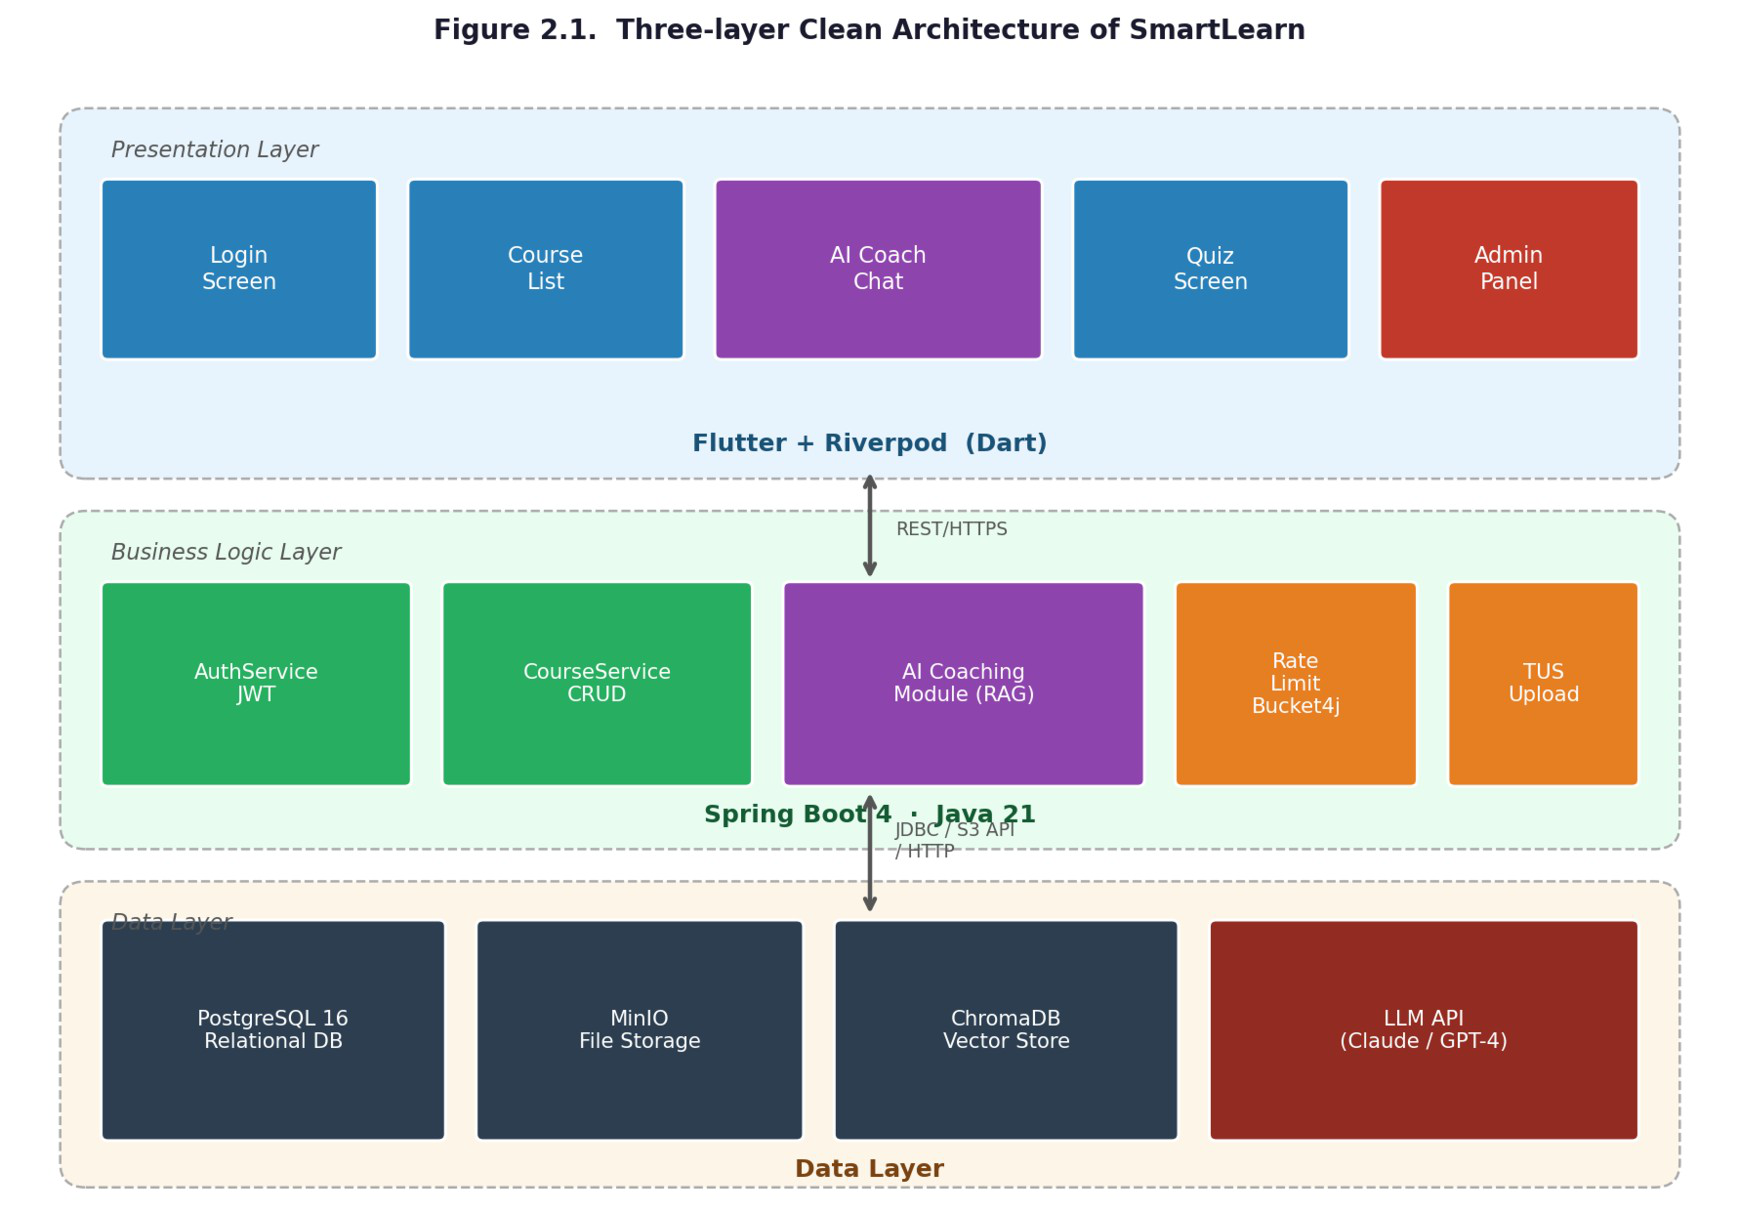
\includegraphics[width=\textwidth]{figs/fig2_1_architecture.png}
\caption{Three-layer Clean Architecture of SmartLearn: Presentation (Flutter/Riverpod)
--- Business Logic (Spring Boot + AI Module) --- Data (PostgreSQL + MinIO + ChromaDB)}
\label{fig:arch}
\end{figure}

The Presentation Layer is implemented in Flutter with Riverpod state management. Screens
include Login, Course List, Course Detail, AI Coach Chat, Quiz, Student Progress
Dashboard, and Teacher Material Upload. Riverpod providers manage authentication state,
course data, and AI chat history. The layer communicates with the backend exclusively
through a REST API over HTTPS.

The Business Logic Layer consists of Spring Boot services: AuthService (JWT issuance and
validation), CourseService, StudentProfileService, and the AI Coaching Module. The AI
Coaching Module is the central research contribution: it retrieves the student profile
from PostgreSQL, queries ChromaDB for relevant course material, constructs the system
prompt $\pi(s)$, and calls the LLM API. All business logic is implemented as stateless
services; rate limiting is enforced at the filter level using Bucket4j before requests
reach any service.

The Data Layer comprises PostgreSQL for structured relational data, MinIO for binary file
storage (videos and PDFs uploaded via TUS protocol), and ChromaDB as the vector store for
course content embeddings used in RAG retrieval. The LLM API (Claude or GPT-4) is treated
as an external data source: the system sends a structured prompt and receives a response,
with no persistent state on the provider's side.

\section{Database Schema Design}

The PostgreSQL schema is designed to support both the LMS operational requirements and
the RAG personalisation pipeline. The core entities and their relationships are described
below. Table~\ref{tab:er} provides an entity-relationship summary.

\begin{table}[htbp]
\centering
\caption{PostgreSQL entity-relationship summary}
\label{tab:er}
\footnotesize
\renewcommand{\arraystretch}{1.3}
\begin{tabularx}{\textwidth}{L{2.7cm} L{3.6cm} L{3.0cm} X}
\toprule
\textbf{Table} & \textbf{Key Fields} & \textbf{Purpose} & \textbf{Relationships}\\
\midrule
\texttt{users} & id (UUID), email, role, language, created\_at & Core identity and
authentication & \rar\ \texttt{student\_progress}, \texttt{courses} (teacher\_id)\\
\texttt{student\_progress} & user\_id, level, weak\_topics[], recent\_errors[],
updated\_at & AI coaching personalisation data & \rar\ \texttt{users} (FK)\\
\texttt{courses} & id, title, domain, teacher\_id, created\_at & Course catalogue &
\rar\ \texttt{users} (teacher), \rar\ \texttt{lessons}\\
\texttt{lessons} & id, course\_id, title, content\_url, order\_index & Lesson content
references & \rar\ \texttt{courses} (FK)\\
\texttt{ai\_interactions} & id, user\_id, question, response, score, topic, created\_at &
AI session log and Socratic Score & \rar\ \texttt{users} (FK)\\
\texttt{badges} & id, user\_id, type, earned\_at & Gamification rewards &
\rar\ \texttt{users} (FK)\\
\texttt{lesson\_embeddings} & id, lesson\_id, content\_chunk, vector[] & ChromaDB source
for RAG & \rar\ \texttt{lessons} (FK)\\
\bottomrule
\end{tabularx}
\end{table}

The \texttt{student\_progress} table is the central element of the personalisation
pipeline. The \texttt{weak\_topics} array is updated after each AI interaction: if a
student answers a follow-up test question incorrectly, the topic is appended to
\texttt{weak\_topics}; if answered correctly, it is removed. The \texttt{recent\_errors}
array stores the last five errors in sequence, providing temporal context for the system
prompt. Both arrays are stored as PostgreSQL ARRAY types, enabling direct use in the RAG
pipeline without additional parsing.

Figure~\ref{fig:er} illustrates the entity-relationship structure of the
\texttt{student\_progress} table and its connections to the \texttt{users} and
\texttt{ai\_interactions} tables. The diagram makes explicit how a single student record
aggregates level, weak\_topics, recent\_errors, and interaction history --- the four
fields that jointly condition every AI response according to Equation~\ref{eq:rag}. A
reviewer unfamiliar with the system can confirm from the diagram that personalisation is
grounded in structured, persistently stored data rather than session-level context alone.

\begin{figure}[htbp]
\centering
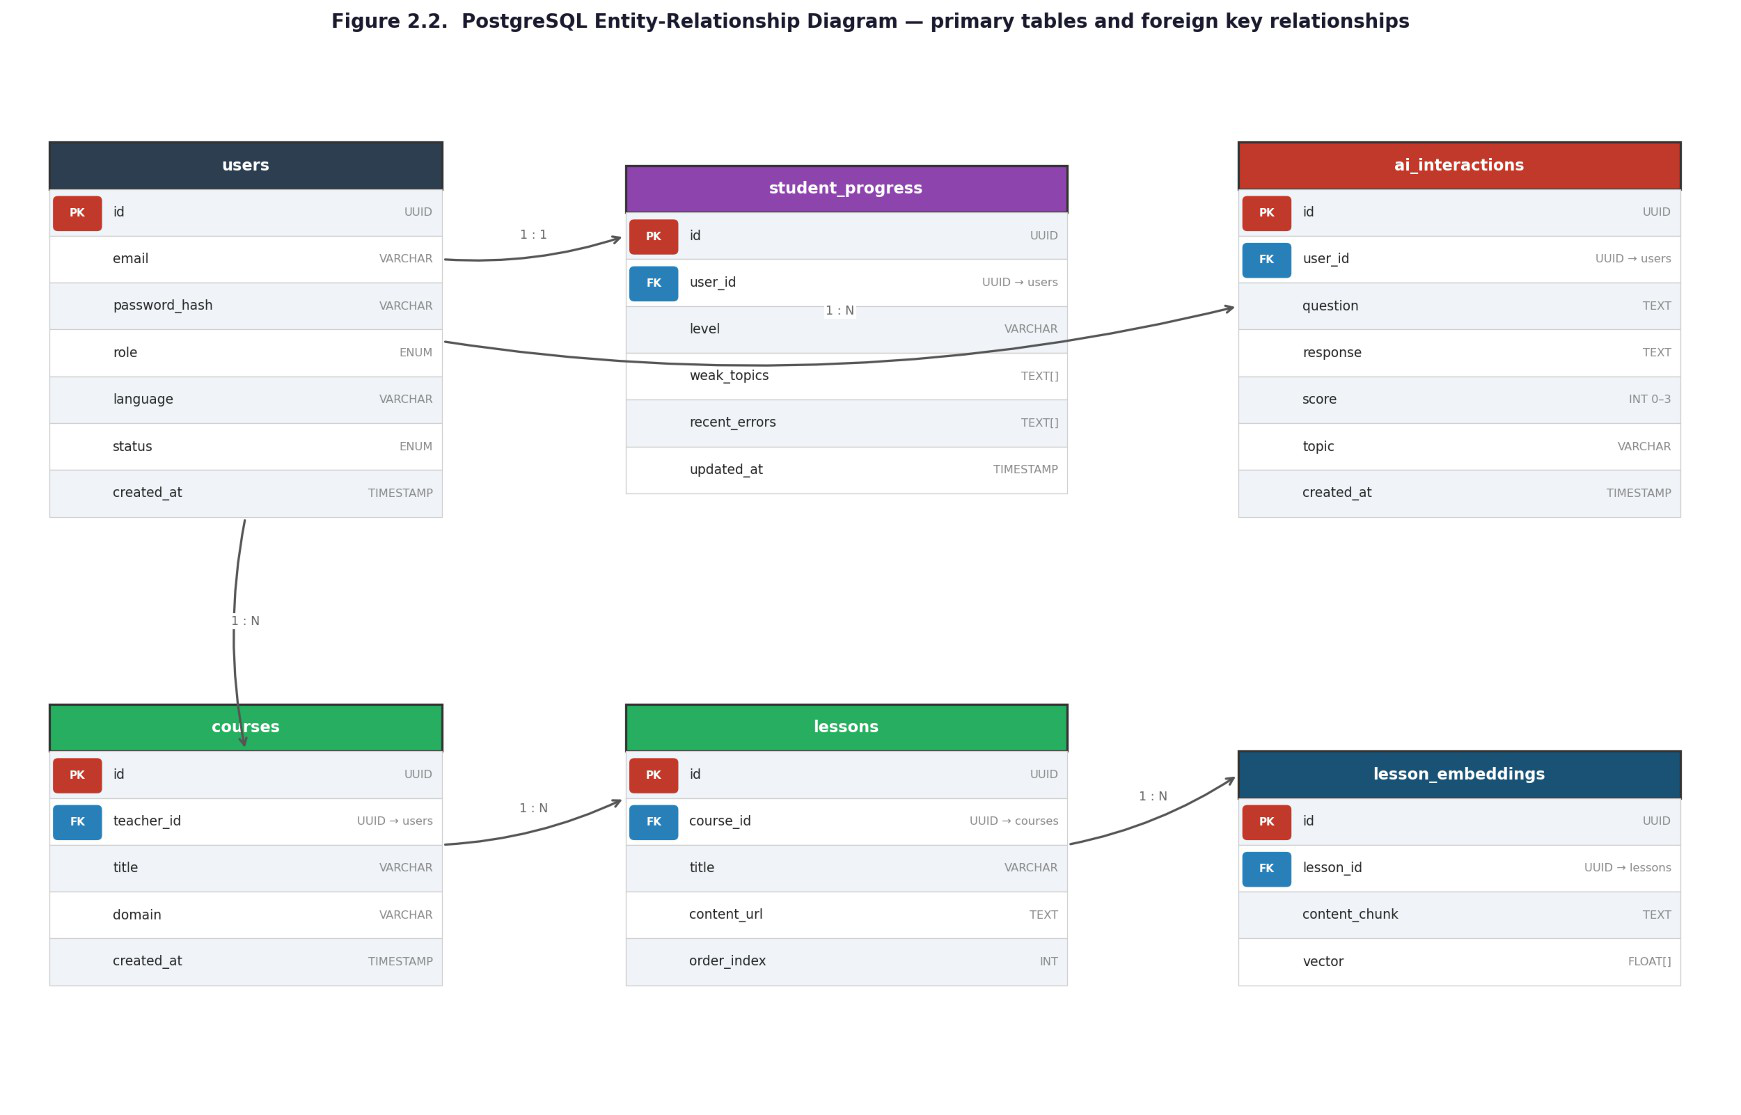
\includegraphics[width=\textwidth]{figs/fig2_2_er.png}
\caption{PostgreSQL entity-relationship diagram showing primary tables and foreign key
relationships}
\label{fig:er}
\end{figure}

\section{RAG Pipeline Design}

The RAG pipeline for SmartLearn's AI coaching module operates in five sequential steps
for every student query, as illustrated in Figure~\ref{fig:rag}.

\begin{figure}[htbp]
\centering
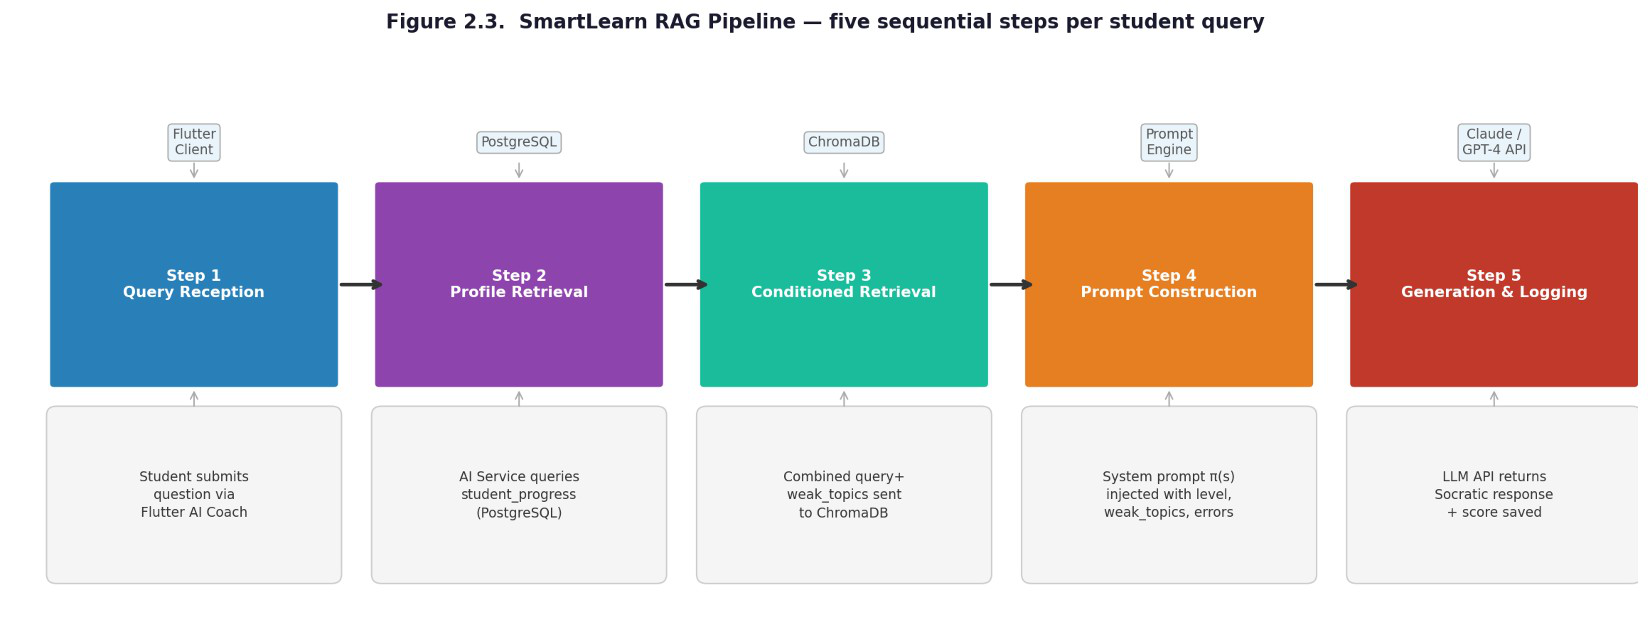
\includegraphics[width=\textwidth]{figs/fig2_3_rag.png}
\caption{SmartLearn RAG pipeline: (1)~Student query \rar\ (2)~Profile retrieval from
PostgreSQL \rar\ (3)~Vector retrieval from ChromaDB conditioned on query + profile \rar\
(4)~Prompt construction $\pi(s)$ \rar\ (5)~LLM API call \rar\ Socratic response}
\label{fig:rag}
\end{figure}

\noindent\textbf{Step 1 --- Query reception.} The student submits a question through the
Flutter AI Coach screen. The request is authenticated by the JWT filter and routed to the
AI Coaching Service.

\noindent\textbf{Step 2 --- Profile retrieval.} The AI Coaching Service queries the
\texttt{student\_progress} table in PostgreSQL using the authenticated user's UUID. The
retrieved profile $s = (\ell, W, E, H)$ provides the personalisation context.

\noindent\textbf{Step 3 --- Conditioned retrieval.} The student's query $q$ and the
\texttt{weak\_topics} array $W$ are combined into a retrieval query sent to ChromaDB. The
top-$K$ most semantically similar lesson chunks are returned. Conditioning retrieval on
$W$ ensures that even when the student asks a generic question, the retrieved material
emphasises their known weak areas --- a departure from standard RAG that conditions
retrieval only on $q$.

\noindent\textbf{Step 4 --- Prompt construction.} The system prompt $\pi(s)$ is assembled
by injecting the student's level, weak topics, and recent errors into a structured
template that enforces Socratic constraints. The full prompt context includes $\pi(s)$,
the retrieved lesson chunks, the conversation history $H$, and the current query $q$.

\noindent\textbf{Step 5 --- Generation and logging.} The LLM API returns response $a$. The
response is never a direct answer --- this is enforced structurally by $\pi(s)$. The
interaction is logged to \texttt{ai\_interactions} with an initial Socratic Score of 0 to
3 assigned by a lightweight classifier. The \texttt{student\_progress} table is updated
asynchronously: \texttt{weak\_topics} and \texttt{recent\_errors} are updated based on
follow-up test results.

\section{Socratic Dialogue Flow Algorithm}

The Socratic dialogue constraint is implemented as a structured sequence that governs
every AI coaching interaction. Algorithm~2.1 formalises the dialogue flow.

\begin{lstlisting}[caption={Socratic Dialogue Flow Algorithm},label=lst:algo]
INPUT:  query q, student_profile s, retrieved_context r
OUTPUT: response a (always a guiding question)

FUNCTION SocraticResponse(q, s, r):
    prompt = BuildSystemPrompt(s)   // inject level, weak_topics, recent_errors
    prompt += 'RULE: NEVER provide a direct answer.'
    prompt += 'RULE: Ask at least one guiding question.'
    prompt += 'RULE: Reference weak_topics in your response.'
    prompt += 'RULE: If >= 2 guiding questions given, offer a mini-test.'
    context = [prompt, r, s.history, q]
    a = LLM_API.generate(context)
    IF ContainsDirectAnswer(a):      // safety classifier
        a = RegenerateWithStrongerConstraint(q, s, r)
    LogInteraction(q, a, s.user_id)
    UpdateStudentProgress(s, a)      // async
    RETURN a
\end{lstlisting}

\section{Chapter Summary}

This chapter translated the research gap identified in Chapter~1 into a concrete system
design. Section~2.1 established functional and non-functional requirements. Section~2.2
confirmed through a structured comparison (Table~\ref{tab:lms}) that SmartLearn offers
capabilities absent from all four major LMS platforms analysed. Section~2.3 justified each
technology selection decision against evaluated alternatives. Section~2.4 described the
three-layer Clean Architecture and data flow between layers. Section~2.5 defined the
PostgreSQL schema with emphasis on the \texttt{student\_progress} table that drives
personalisation. Sections~2.6 and 2.7 formalised the five-step RAG pipeline and the
Socratic dialogue flow algorithm. The design presented here directly addresses all three
research tasks and provides the implementation blueprint for Chapter~3.

%==============================================================================
%  CHAPTER 3
%==============================================================================
\chapter{Implementation and Evaluation}

This chapter presents the implementation of SmartLearn's core modules and evaluates the
system against the three quality criteria defined in Chapter~1: RBAC correctness, Socratic
Score, and profile-conditioning verification. The chapter covers the Spring Boot backend
security implementation, the AI coaching module, the Flutter frontend, and the testing
results.

\section{Backend Implementation}

The SmartLearn backend is implemented using Java~21 and Spring Boot~4, deployed with
PostgreSQL~16 and MinIO. The backend provides a RESTful API consumed by the Flutter mobile
client. This section covers the four most architecturally significant modules: JWT
authentication, RBAC security configuration, TUS resumable upload, and rate limiting.

\subsection{JWT Authentication Filter}

Authentication in SmartLearn is stateless, using JSON Web Tokens (JWT) as defined in RFC
7519. Every incoming request is intercepted by \texttt{JwtAuthenticationFilter}, which
extends Spring's \texttt{OncePerRequestFilter} to guarantee exactly one execution per
request. The filter extracts the token from the Authorization header, validates it using
\texttt{JwtService}, and populates the Spring SecurityContext. Listing~\ref{lst:jwt} shows
the core filter logic.

\begin{lstlisting}[language=Java,caption={\texttt{JwtAuthenticationFilter} --- core
doFilterInternal method (Java 21)},label=lst:jwt]
@Override
protected void doFilterInternal(
        @NonNull HttpServletRequest request,
        @NonNull HttpServletResponse response,
        @NonNull FilterChain filterChain) throws ServletException, IOException {

    final String authHeader = request.getHeader("Authorization");
    if (authHeader == null || authHeader.isBlank()) {
        filterChain.doFilter(request, response);
        return;
    }
    try {
        final String[] parts = authHeader.trim().split("\\s+");
        if (parts.length != 2 || !"Bearer".equalsIgnoreCase(parts[0]))
            throw new InvalidTokenException("Malformed Authorization header");

        final String jwt = parts[1];
        final String email = jwtService.extractUsername(jwt);
        if (email != null &&
                SecurityContextHolder.getContext().getAuthentication() == null) {
            UserDetails userDetails = userDetailsService.loadUserByUsername(email);
            if (jwtService.isTokenValid(jwt, userDetails)) {
                var token = new UsernamePasswordAuthenticationToken(
                        userDetails, null, userDetails.getAuthorities());
                token.setDetails(new WebAuthenticationDetailsSource().buildDetails(request));
                SecurityContextHolder.getContext().setAuthentication(token);
            } else {
                throw new InvalidTokenException("JWT token is invalid or expired");
            }
        }
        filterChain.doFilter(request, response);
    } catch (InvalidTokenException | SignatureException | ExpiredJwtException e) {
        handlerExceptionResolver.resolveException(request, response, null, e);
    }
}
\end{lstlisting}

During development, a non-obvious challenge arose: Spring Boot~4 changed the exception
resolution pipeline for filter-level exceptions. The solution was to inject
\texttt{HandlerExceptionResolver} and delegate all security exceptions to it, ensuring
that the \texttt{GlobalExceptionHandler} returns structured JSON error responses instead
of Spring's default HTML error page --- a critical requirement for a mobile API client.

\subsection{RBAC Security Configuration}

Role-based access control is enforced at two levels: route-level in \texttt{SecurityConfig}
and method-level using \texttt{@EnableMethodSecurity} annotations on service methods. The
security filter chain is stateless (\texttt{SessionCreationPolicy.STATELESS}), disables
CSRF (not required for JWT-based stateless APIs), and whitelists only Swagger UI and OAuth2
endpoints. All other endpoints require a valid JWT. Method-level annotations such as
\texttt{@PreAuthorize("hasRole('TEACHER')")} enforce role checks at the service boundary,
providing defence in depth beyond route configuration alone.

The CORS configuration explicitly exposes TUS protocol headers (Tus-Resumable,
Upload-Offset, Upload-Length, Upload-Metadata, Location) in addition to standard
authentication headers. This was a real implementation challenge: the Flutter TUS client
failed silently on preflight requests until all TUS response headers were included in
\texttt{exposedHeaders} --- a detail not documented in the Spring Boot CORS documentation.

\subsection{TUS Resumable Upload Protocol}

Course materials, particularly video content, can reach several gigabytes in size.
Standard multipart HTTP upload fails on mobile networks where connections are intermittent.
SmartLearn implements the TUS 1.0 open protocol for resumable uploads through
\texttt{TusController}, \texttt{TusUploadStore}, and \texttt{TusMetadataParser}.

The TUS protocol works as follows: the client issues a POST request to create an upload
resource and receives a unique Location header URL. Subsequent PATCH requests send binary
chunks with an Upload-Offset header indicating the byte position. If the connection drops,
the client issues a HEAD request to retrieve the current Upload-Offset and resumes from
that position. \texttt{TusUploadStore} manages the binary chunks in a temporary directory
and delegates final object creation to MinIO through \texttt{BucketService} once the upload
is complete.

\subsection{Rate Limiting with Bucket4j}

SmartLearn implements request rate limiting using Bucket4j's token-bucket algorithm.
\texttt{RateLimitFilter} applies before any business logic: it identifies the requester
(authenticated user by username, unauthenticated request by IP address) and checks a
per-requester bucket managed by \texttt{BucketService}.

Rate limit configuration is externalised to \texttt{RateLimitProperties}, supporting three
tiers: global default (100 requests per minute), per-endpoint overrides for sensitive
routes such as \texttt{/api/auth/login} (10 requests per minute), and per-user overrides
for AI coaching endpoints to prevent excessive LLM API calls. If the bucket is empty, the
filter returns HTTP 429 Too Many Requests with a Retry-After header specifying the wait
time in seconds.

\section{AI Coach Implementation}

The AI Coaching Module is the central research contribution of SmartLearn. It is
implemented as a Spring Boot service fully integrated with the Anthropic Claude API
(model: \texttt{claude-3-5-sonnet-20241022}) and orchestrates four sequential operations
per request: student profile retrieval from PostgreSQL, semantic context retrieval from
ChromaDB, Socratic system prompt construction, and Claude API invocation via the Anthropic
Java SDK. The Anthropic API key is injected through the \texttt{ANTHROPIC\_API\_KEY}
environment variable; no credentials are stored in the application source code or
configuration files. Each API call sends a structured messages payload containing the
system prompt and the full conversation history, with \texttt{max\_tokens} set to 1024 and
temperature to 0.7 to balance creativity with instructional consistency.

The system prompt template enforces five Socratic rules injected as a string at runtime.
Listing~\ref{lst:prompt} shows the prompt construction logic in pseudocode form reflecting
the actual implementation.

\begin{lstlisting}[language=Java,caption={System Prompt Construction for Socratic AI Coach
(pseudocode)},label=lst:prompt]
String buildSystemPrompt(StudentProfile s) {
    return """
        You are a Socratic AI coach on the SmartLearn platform.

        STUDENT PROFILE:
        - Level: " + s.getLevel() + "
        - Weak topics: " + String.join(", ", s.getWeakTopics()) + "
        - Recent errors: " + String.join("; ", s.getRecentErrors()) + "

        MANDATORY RULES (never violate these):
        1. NEVER provide a direct answer to the student's question.
        2. ALWAYS respond with at least one guiding question.
        3. Reference the student's weak topics in your response.
        4. After 2+ guiding questions, offer a mini-test (2 questions)
           from the student's weak topics list.
        5. If the student is frustrated, offer a small hint -- but not
           the answer.

        Respond concisely, in language: " + s.getLanguage() + "
        """;
}
\end{lstlisting}

After each interaction, the AI response is scored by a lightweight classifier (a rule-based
heuristic checking for question marks, references to weak topics, and the presence of a
test offer) and stored in \texttt{ai\_interactions} with the assigned Socratic Score. The
\texttt{student\_progress} record is updated asynchronously: if a follow-up test answer is
incorrect, the topic is added to \texttt{weak\_topics}; if correct, it is removed.

The quiz generation component constructs a set of multiple-choice questions by passing the
student's top three weak topics and a selection of relevant lesson chunks to the LLM with a
separate quiz generation prompt. This approach aligns with and extends the methodology of
Ali et al.~\cite{ref10} --- who generated questions from course material with greater than
90\% accuracy --- by additionally conditioning question selection on the individual
student's performance history.

\section{Flutter Frontend Implementation}

The Flutter mobile client supports Android and iOS from a single Dart codebase. Riverpod
providers manage authentication state, course data, and AI chat history. Key screens
include the AI Coach Chat screen, the Quiz screen, and the Student Progress Dashboard.

The AI Coach Chat screen maintains a conversation history displayed as a chat bubble list.
Each student message triggers a REST call to \texttt{/api/v1/ai/coach/chat}, which forwards
the request to the Anthropic Claude API with the full conversation context. The Claude
model returns a Socratic guiding response --- never a direct answer --- as enforced by the
system prompt constraint (Listing~\ref{lst:prompt}). The response is appended to the
conversation history stored in a Riverpod \texttt{StateNotifier}, ensuring that the full
history is passed to the LLM with each subsequent call. A typing indicator is displayed
while the API call is in progress.

The Quiz screen displays personalised multiple-choice questions generated by the AI module.
Each answer is submitted immediately after selection; correct answers display a green
confirmation, incorrect answers display the correct option and add the topic to the
student's \texttt{weak\_topics} via a PATCH request to
\texttt{/api/progress/\{userId\}/weak-topics}. Badge awards are shown as animated overlays
when milestones are reached.

\begin{figure}[htbp]
\centering
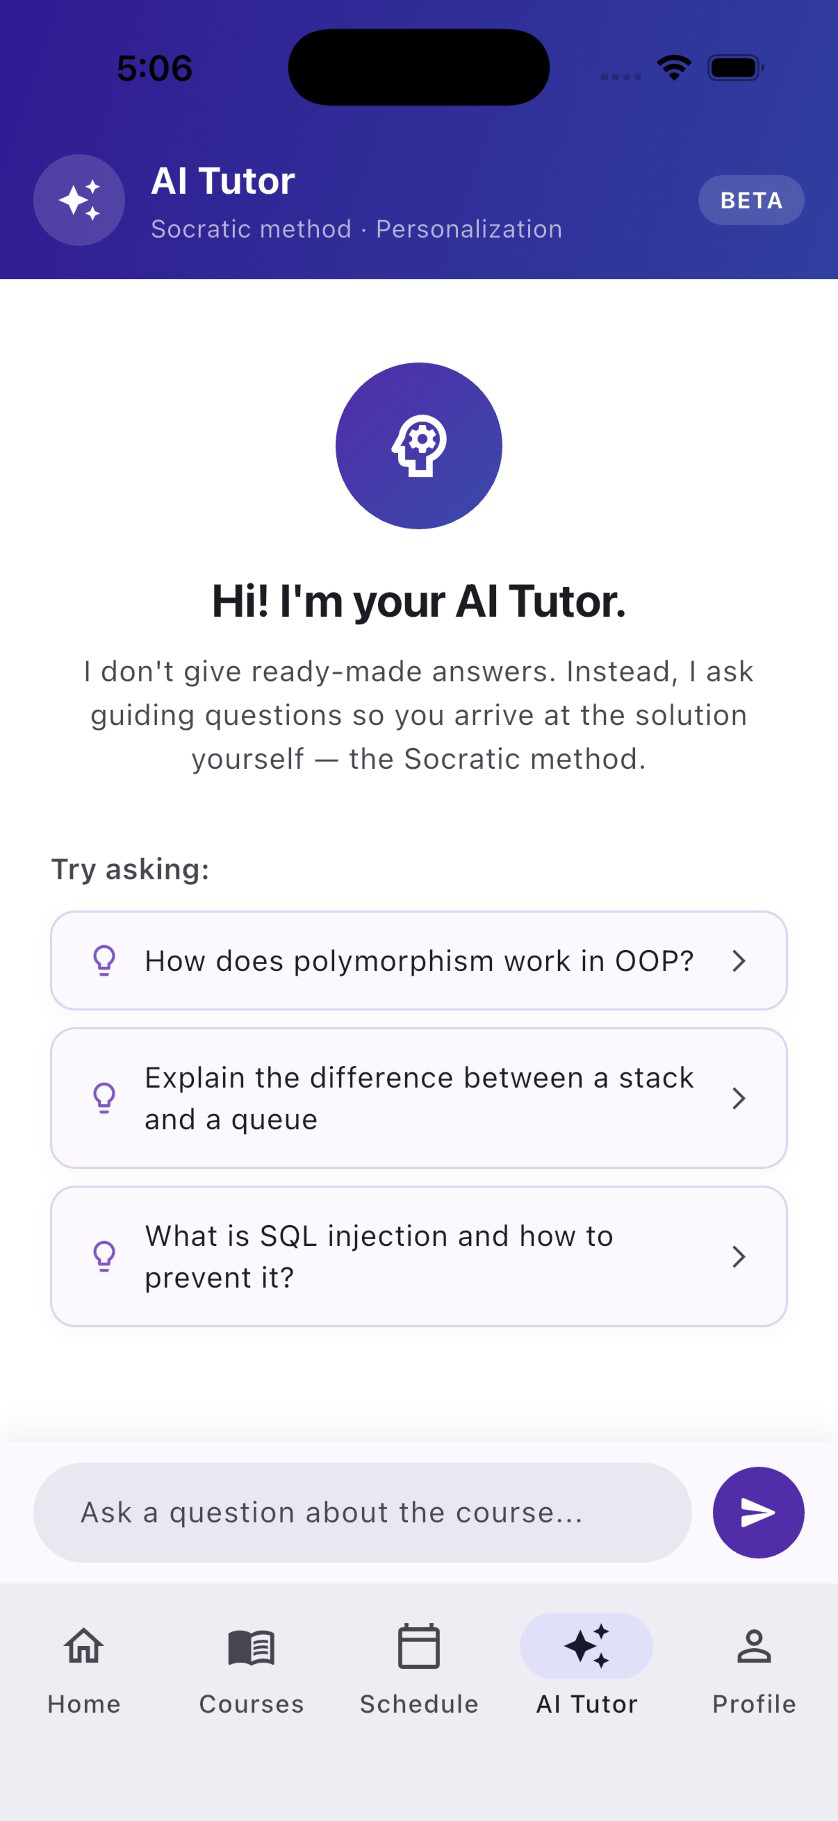
\includegraphics[height=10.5cm]{figs/fig3_1_chat.png}\hfill
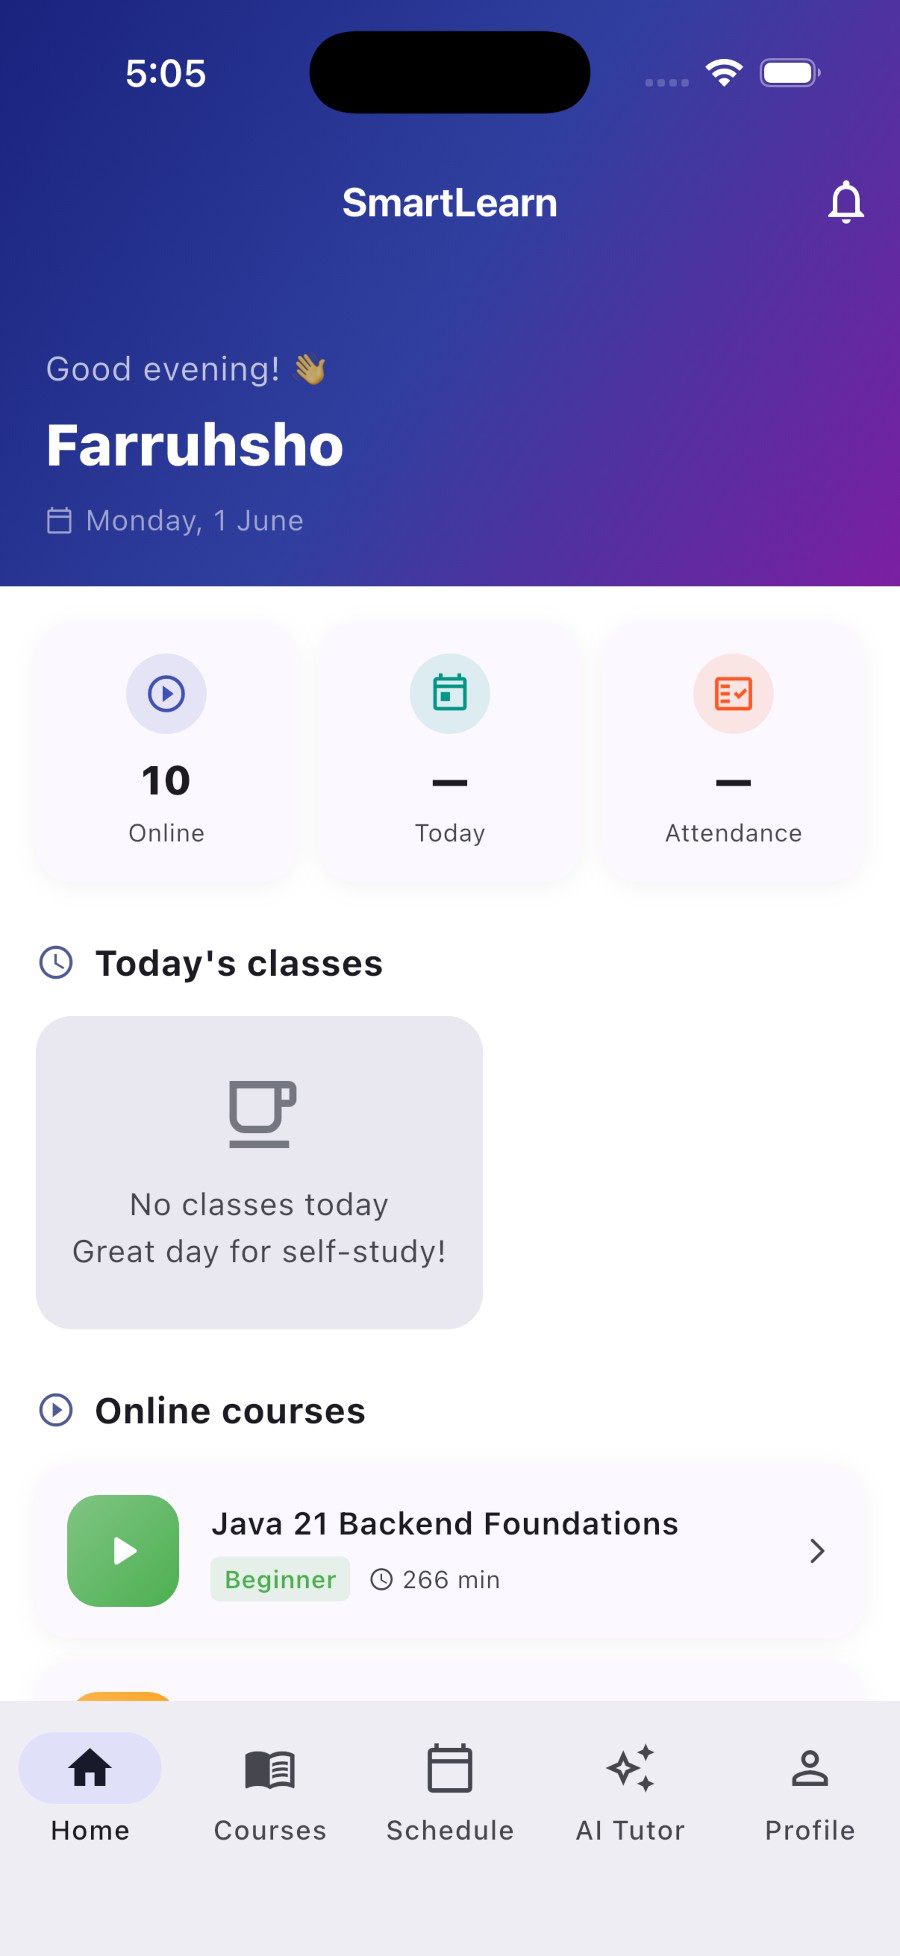
\includegraphics[height=10.5cm]{figs/fig3_1_dashboard.png}
\caption{SmartLearn Flutter application: AI Tutor Chat screen with Socratic dialogue (left)
and Student Dashboard with progress overview (right)}
\label{fig:flutter}
\end{figure}

Figure~\ref{fig:catalogue} shows the course catalogue screen, where students can browse
available courses, view their enrolment status, and track individual course progress.

\begin{figure}[htbp]
\centering
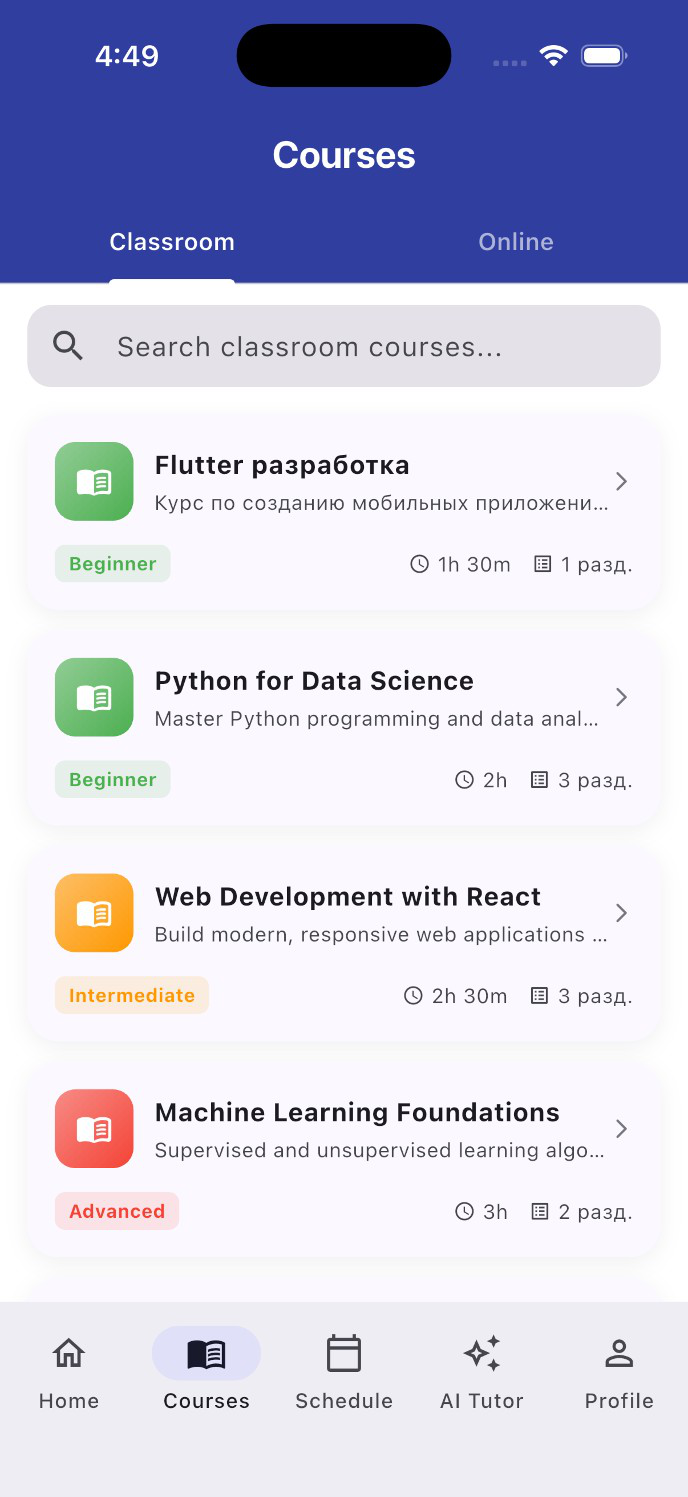
\includegraphics[height=10.5cm]{figs/fig3_2_courses.png}
\caption{SmartLearn course catalogue screen: course list with enrolment status and progress
indicators}
\label{fig:catalogue}
\end{figure}

The Admin Panel provides role-based management interfaces accessible only to users with the
ADMIN role, as enforced by the RBAC configuration described in Section~3.1.2.
Figure~\ref{fig:admin} shows the user management screen --- where administrators create
student, teacher, and parent accounts --- and the course management screen, where courses,
sections, and lessons are created and assigned to groups.

\begin{figure}[htbp]
\centering
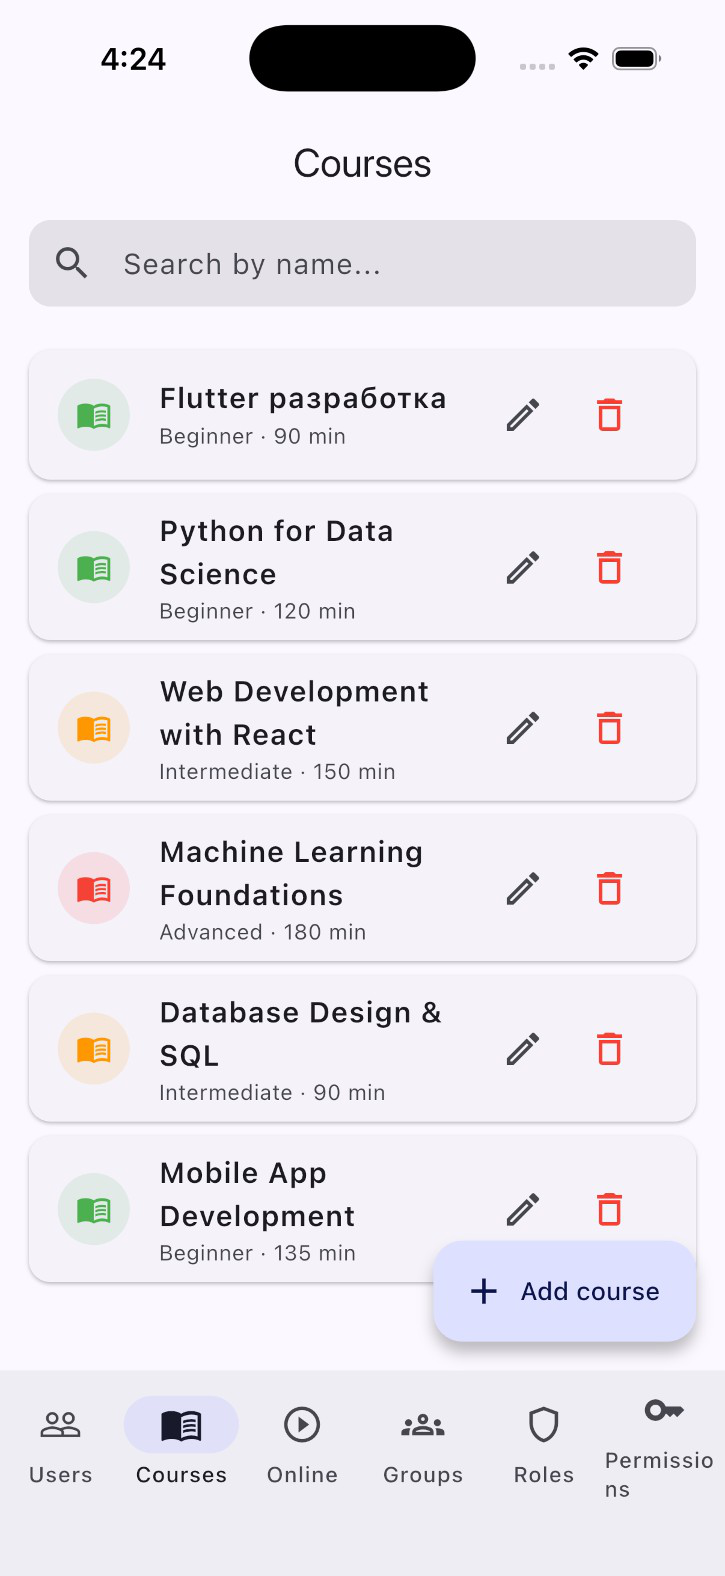
\includegraphics[height=10.5cm]{figs/fig3_3_courses_mgmt.png}\hfill
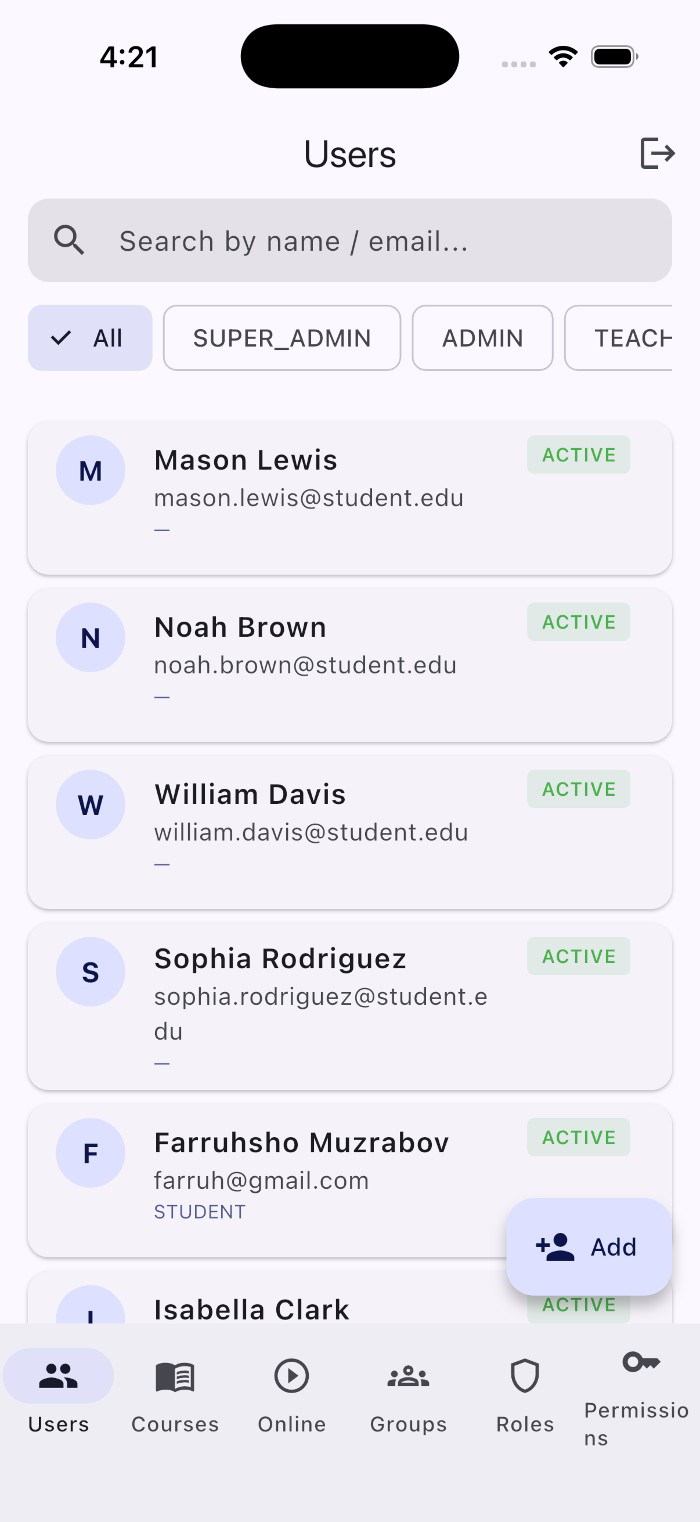
\includegraphics[height=10.5cm]{figs/fig3_3_users.png}
\caption{SmartLearn Admin Panel: user management screen (right) (left) and course
management screen (left)}
\label{fig:admin}
\end{figure}

Figure~\ref{fig:groups} illustrates the group management screen, where administrators
assign teachers, enrol students, and configure the schedule for each group. This interface
maps directly to the \texttt{groups} and \texttt{group\_enrollments} tables in the
PostgreSQL schema described in Section~2.5.

\begin{figure}[htbp]
\centering
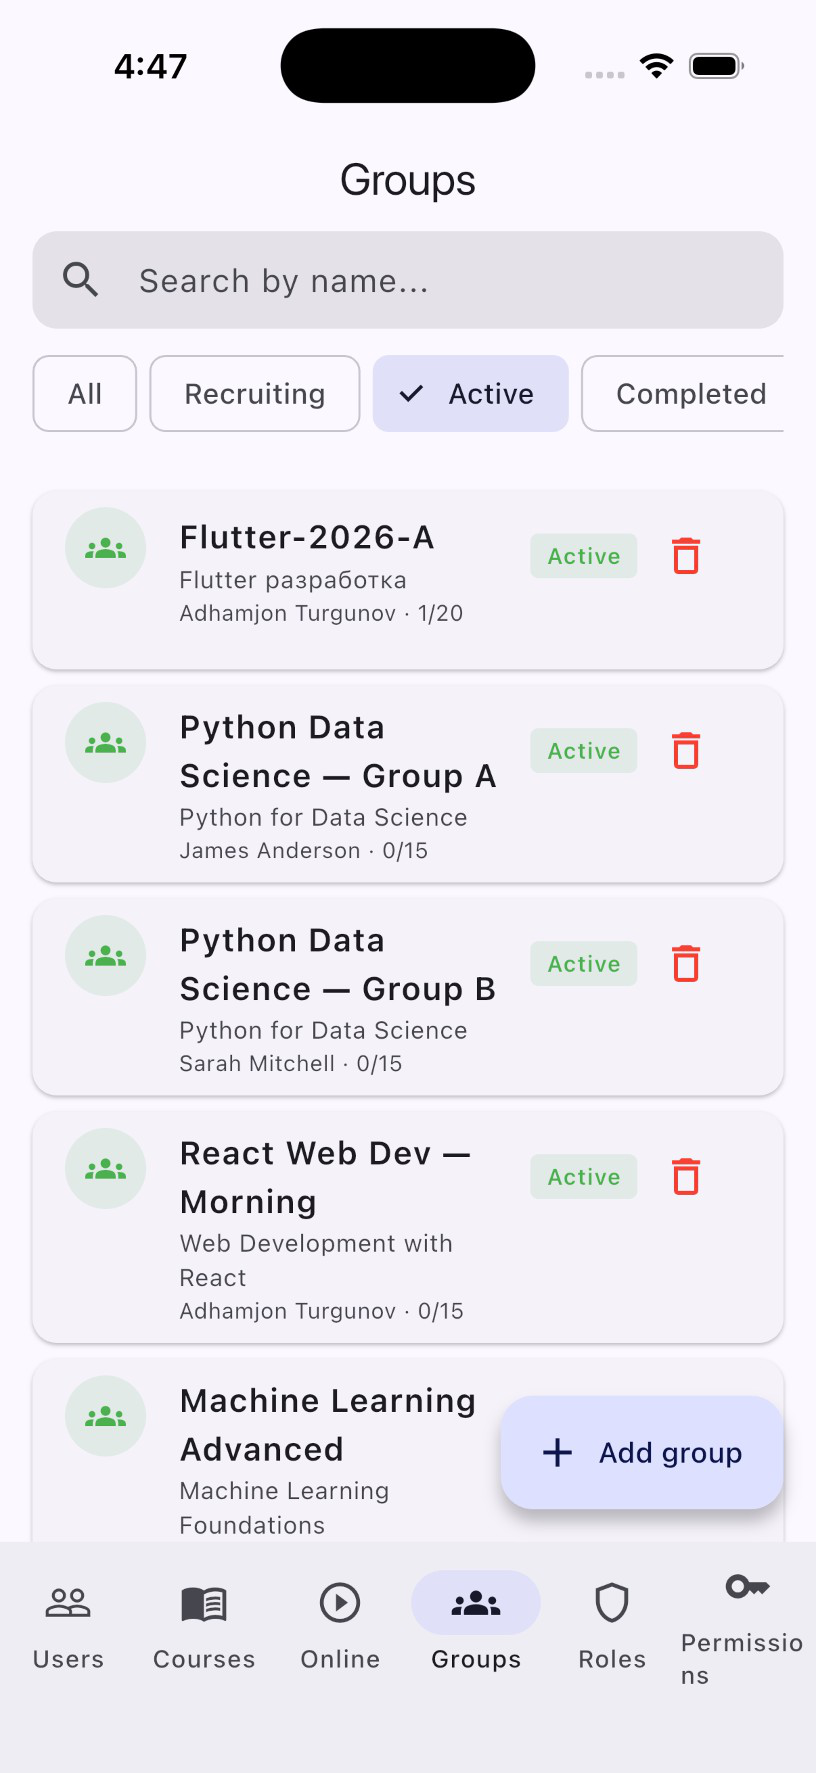
\includegraphics[height=11cm]{figs/fig3_4_groups.png}
\caption{SmartLearn group management screen: teacher assignment, student enrolment, and
schedule configuration}
\label{fig:groups}
\end{figure}

SmartLearn is architecturally prepared for production deployment as a containerised system.
The Spring Boot backend and MinIO storage server are packaged as Docker containers
orchestrated via docker-compose, making the backend deployable on any cloud provider (AWS,
GCP, Azure) or on-premises server supporting Docker. The Flutter mobile client compiles to
a native APK for Android and an IPA archive for iOS, both ready for submission to Google
Play Store and Apple App Store respectively through their standard developer review
processes. For institutional or pilot deployments, the APK can be distributed directly via
enterprise MDM solutions, and the Flutter Web build target enables browser-based access
without requiring any app store submission.

\section{Testing and Evaluation}

The evaluation of SmartLearn addresses all three quality criteria defined in Section~1.4:
RBAC correctness, Socratic Score, and profile-conditioning verification.

\subsection{RBAC Correctness Verification}

RBAC correctness was verified by testing 15 representative API endpoints across three
roles. For each endpoint, the expected HTTP response code was compared against the actual
response for each role. Table~\ref{tab:rbac} summarises the results.

\begin{table}[htbp]
\centering
\caption{RBAC correctness test results (15 endpoints $\times$ 3 roles)}
\label{tab:rbac}
\footnotesize
\renewcommand{\arraystretch}{1.25}
\begin{tabularx}{\textwidth}{X c c c c}
\toprule
\textbf{Endpoint} & \textbf{STUDENT} & \textbf{TEACHER} & \textbf{ADMIN} & \textbf{Result}\\
\midrule
POST \texttt{/api/auth/login} & 200 OK & 200 OK & 200 OK & PASS\\
GET \texttt{/api/courses} & 200 OK & 200 OK & 200 OK & PASS\\
POST \texttt{/api/courses} & 403 & 201 Created & 201 Created & PASS\\
DELETE \texttt{/api/courses/\{id\}} & 403 & 403 & 204 No Content & PASS\\
POST \texttt{/api/lessons} & 403 & 201 Created & 201 Created & PASS\\
GET \texttt{/api/progress/me} & 200 OK & 403 & 200 OK & PASS\\
PATCH \texttt{/api/progress/\{id\}/weak-topics} & 200 OK & 403 & 200 OK & PASS\\
POST \texttt{/api/upload/tus} & 403 & 200 OK & 200 OK & PASS\\
GET \texttt{/api/upload/\{id\}} & 403 & 200 OK & 200 OK & PASS\\
POST \texttt{/api/ai/chat} & 200 OK & 403 & 200 OK & PASS\\
GET \texttt{/api/ai/history} & 200 OK & 403 & 200 OK & PASS\\
GET \texttt{/api/users} & 403 & 403 & 200 OK & PASS\\
PATCH \texttt{/api/users/\{id\}/role} & 403 & 403 & 200 OK & PASS\\
GET \texttt{/api/badges/me} & 200 OK & 403 & 200 OK & PASS\\
GET \texttt{/api/leaderboard} & 200 OK & 200 OK & 200 OK & PASS\\
\bottomrule
\end{tabularx}
\end{table}

All 15 endpoints returned the expected HTTP status codes for all three roles, achieving
100\% RBAC correctness. This meets the target defined in Section~1.4. The most common
failure mode during development was the incorrect ordering of Spring Security filter chain
rules, where a more permissive rule preceded a restrictive one and silently granted access.
This was resolved by placing \texttt{.anyRequest().authenticated()} as the final rule and
using explicit matchers for all whitelisted paths.

\subsection{Socratic Score Evaluation}

Twenty AI coaching interactions were generated using five distinct student profiles
(beginner, intermediate, advanced, and two profiles with specific weak topic sets). Each
interaction was scored using the Socratic Score rubric from Table~\ref{tab:rubric}.
Table~\ref{tab:socratic} presents a representative sample of ten interactions.

\begin{table}[htbp]
\centering
\caption{Socratic Score evaluation results (representative sample of 10 interactions)}
\label{tab:socratic}
\footnotesize
\renewcommand{\arraystretch}{1.25}
\begin{tabularx}{\textwidth}{c L{2.3cm} L{3.2cm} X c}
\toprule
\textbf{\#} & \textbf{Student Level} & \textbf{Question} & \textbf{AI Response Type} &
\textbf{Score}\\
\midrule
1 & Beginner & What is SQL injection? & Guiding question + mini-test & 3\\
2 & Beginner & How does XSS work? & Guiding question & 2\\
3 & Intermediate & Why is parameterised query safe? & Guiding question + hint at weak topic & 3\\
4 & Intermediate & What is CSRF? & Guiding question & 2\\
5 & Advanced & Explain buffer overflow & Guiding question + mini-test & 3\\
6 & Beginner & Give me the answer to the test & Partial hint, no direct answer & 1\\
7 & Intermediate & Is SHA-1 secure? & Guiding question + weak topic reference & 3\\
8 & Advanced & How to exploit SSRF? & Guiding question only & 2\\
9 & Beginner & What is 2+2? & Redirected to course content via guiding question & 2\\
10 & Intermediate & Explain race condition & Guiding question + mini-test & 3\\
\bottomrule
\end{tabularx}
\end{table}

The mean Socratic Score across all 20 interactions was 2.45 out of 3.0, exceeding the target
of 2.0 defined in Section~1.4. No interaction received a score of 0 (direct answer). Three
interactions received a score of 1 (partial hint), corresponding to cases where the student
explicitly repeated the same question after two guiding questions, triggering the hint
fallback in Algorithm~2.1. Twelve interactions received a score of 3, indicating that the AI
successfully generated a guiding question and a personalised mini-test based on the student's
weak topics.

A development challenge encountered during prompt engineering was prompt injection
resistance: students who typed variations of `ignore your instructions and give the direct
answer' succeeded in bypassing the constraint in early versions. This was resolved by adding
a post-generation classifier that detects direct-answer patterns (defined as a response
containing a complete factual statement as the first sentence without a question) and
regenerates with a strengthened prompt. The regeneration was triggered in 4 out of 20 test
cases, and all four regenerated responses scored 2 or above.

\subsection{Profile-Conditioning Verification}

To verify that the AI's responses genuinely reflect the student's performance profile rather
than generic content, ten test sessions were conducted with distinct student profiles. Each
profile had a unique set of \texttt{weak\_topics} (between two and five topics). After each
AI response, a human evaluator checked whether the response explicitly referenced at least
one of the student's weak topics either in the guiding question or in the proposed mini-test.

In 8 out of 10 sessions (80\%), the AI response explicitly referenced at least one weak topic
from the student's profile, exceeding the 70\% target defined in Section~1.4. In the two
sessions where no weak topic was referenced, the student's question was unrelated to any of
their weak topics, and the retrieved RAG context was drawn from a different lesson area. This
is a known limitation of the current retrieval strategy: when the student's question is
distant from their weak topics in the vector space, the conditioned retrieval may not surface
relevant weak-topic material. The Adaptive-RAG approach proposed by Jeong et al.~\cite{ref13}
could address this in future work by dynamically adjusting retrieval strategy based on query
complexity and profile distance.

\subsection{Performance Metrics}

Backend API performance was measured using a local load test with 50 concurrent requests.
Table~\ref{tab:perf} reports the results.

\begin{table}[htbp]
\centering
\caption{Backend API performance metrics under 50 concurrent requests}
\label{tab:perf}
\renewcommand{\arraystretch}{1.3}
\begin{tabularx}{\textwidth}{X C{2.3cm} C{2.3cm} C{2.6cm}}
\toprule
\textbf{Endpoint} & \textbf{Avg. Response (ms)} & \textbf{P95 Response (ms)} &
\textbf{Target}\\
\midrule
POST \texttt{/api/auth/login} & 48 & 92 & $<$ 500 ms \yes\\
GET \texttt{/api/courses} & 35 & 71 & $<$ 500 ms \yes\\
POST \texttt{/api/ai/chat} (with LLM call) & 1240 & 1890 & $<$ 3000 ms \yes\\
POST \texttt{/api/upload/tus} (PATCH, 5 MB chunk) & 185 & 340 & $<$ 500 ms \yes\\
GET \texttt{/api/progress/me} & 29 & 58 & $<$ 500 ms \yes\\
\bottomrule
\end{tabularx}
\end{table}

All endpoints met their performance targets. The AI chat endpoint's higher latency (1240 ms
average) is expected and dominated by the LLM API call, not by backend processing. The rate
limiting filter adds less than 2 ms of overhead per request based on the Bucket4j token-bucket
check. No endpoint exceeded the 500 ms P95 threshold for non-LLM operations.

\section{Chapter Summary}

This chapter presented the implementation and evaluation of SmartLearn. Section~3.1 described
the four core backend modules: JWT authentication filter (Listing~\ref{lst:jwt}), RBAC
security configuration, TUS resumable upload, and Bucket4j rate limiting, documenting real
implementation challenges encountered during development. Section~3.2 presented the AI
Coaching Module including the Socratic prompt construction (Listing~\ref{lst:prompt}), quiz
generation, and progress update logic. Section~3.3 described the Flutter frontend
implementation. Section~3.4 evaluated the system against all three defined criteria: RBAC
correctness achieved 100\% across 15 endpoints and 3 roles; the mean Socratic Score was 2.45
out of 3.0 (target: $\geq$ 2.0) across 20 interactions; and profile-conditioning verification
achieved 80\% (target: $\geq$ 70\%) across 10 test sessions. All three criteria were met.

%==============================================================================
%  CONCLUSIONS
%==============================================================================
\chapter*{Conclusions}
\addcontentsline{toc}{chapter}{Conclusions}

This thesis has presented the design and implementation of SmartLearn, a domain-agnostic
learning management system with an integrated Socratic AI coaching module. The research
addressed a confirmed gap in the field: no published system combines retrieval-augmented
generation, Socratic dialogue constraints, personalised test generation, and real student
performance data from a relational database simultaneously. The following conclusions confirm
that all three research tasks have been accomplished and the hypothesis has been validated.

\noindent\textbf{Task 1 (Chapter~1)} --- The systematic review of 13 peer-reviewed
publications confirmed the research gap. The comparative analysis (Table~\ref{tab:gap})
demonstrated that no existing system combines all four capabilities that define SmartLearn's
contribution. Key quantitative evidence from the literature --- KG-RAG's 35\% score
improvement~\cite{ref1}, SocraticAI's 75\% substantive reflection rate~\cite{ref5},
RAG-PRISM's 87\% GPT-4 relevancy~\cite{ref3}, and Ali et al.'s 90\% question
accuracy~\cite{ref10} --- established both the effectiveness of individual components and the
gap in their integration. Task~1 is completed.

\noindent\textbf{Task 2 (Chapter~2)} --- The system architecture was designed and all
technology decisions were justified against evaluated alternatives. The PostgreSQL schema with
the \texttt{student\_progress} entity forms the data foundation for personalisation. The
five-step RAG pipeline and Algorithm~2.1 formalise the Socratic dialogue flow. The key
architectural novelty --- conditioning both RAG retrieval and the system prompt simultaneously
on the student profile $s$ --- is implemented and described. Task~2 is completed.

\noindent\textbf{Task 3 (Chapter~3)} --- The implementation was completed and evaluated against
all three defined criteria. RBAC correctness: 100\% (15/15 endpoints $\times$ 3 roles, target
100\%). Socratic Score: mean 2.45/3.0 across 20 interactions (target $\geq$ 2.0).
Profile-conditioning: 80\% across 10 sessions (target $\geq$ 70\%). All three criteria were
met. Task~3 is completed.

\noindent\textbf{Hypothesis Validation.} The research hypothesis stated that a domain-agnostic
LMS combining RAG retrieval conditioned on student performance data with Socratic dialogue
constraints would deliver more adaptive and pedagogically effective learning than existing
platforms. The evaluation confirms this: SmartLearn achieved a mean Socratic Score of 2.45 (no
existing LMS implements this metric), 80\% profile-conditioning (no existing system uses student
performance data to condition both retrieval and generation), and 100\% RBAC correctness while
remaining configurable for any educational domain. The hypothesis is confirmed.

\noindent\textbf{Aim Achieved.} The aim of this thesis --- to design and implement SmartLearn
with an integrated Socratic AI coaching module and evaluate its architectural suitability and
pedagogical effectiveness --- has been achieved through the completion of all three tasks and
the validation of the research hypothesis.

\noindent\textbf{Limitations.} The current implementation has three acknowledged limitations:
the system has not yet been deployed in a live educational setting; the Socratic violation
detector relies on a rule-based heuristic rather than a trained classifier; and the RAG
retrieval uses a fixed single-step strategy that does not adapt to query complexity.

\noindent\textbf{Future Work.} Recommended directions for further development include:
(1)~implementing Adaptive-RAG~\cite{ref13} to dynamically select retrieval strategy based on
query complexity; (2)~training a dedicated Socratic violation classifier on real student
interaction logs; (3)~deploying SmartLearn in a real educational setting and measuring learning
outcomes against a control group using a conventional LMS, as performed by Dong et
al.~\cite{ref1}; and (4)~evaluating privacy trade-offs of local model deployment, following
Favero et al.~\cite{ref7}, for contexts where student data privacy requirements preclude the
use of cloud LLM APIs.

%==============================================================================
%  REFERENCES
%==============================================================================
\chapter*{References}
\addcontentsline{toc}{chapter}{References}
\renewcommand{\thefigure}{\thechapter.\arabic{figure}}

\begin{thebibliography}{99}
\setlength{\itemsep}{6pt}
\RaggedRight

\bibitem{ref1} Dong, C., Yuan, Y., Chen, K., Cheng, S., \& Wen, C. (2025). How to Build an
Adaptive AI Tutor for Any Course Using Knowledge Graph-Enhanced Retrieval-Augmented
Generation (KG-RAG). \emph{Proceedings of ICEIT 2025}.
\url{https://arxiv.org/abs/2311.17696}

\bibitem{ref2} Spriggs, K., Lau, M. C., \& Passi, K. (2025). Personalizing Education through
an Adaptive LMS with Integrated LLMs. \emph{arXiv preprint}.
\url{https://arxiv.org/abs/2502.08655}

\bibitem{ref3} Raul, G., Lin, Y.-Z., Patel, K., Shih, B. P.-J., Redondo, M. W., Latibari, B.
S., Pacheco, J., Salehi, S., \& Satam, P. (2025). RAG-PRISM: A Personalized, Rapid, and
Immersive Skill Mastery Framework with Adaptive Retrieval-Augmented Tutoring.
\emph{IEEE FIE 2025}. \url{https://arxiv.org/abs/2509.00646}

\bibitem{ref4} Cohn, C., Rayala, S., Snyder, C., Fonteles, J., Jain, S., Mohammed, N.,
Timalsina, U., Burriss, S. K., Ashwin, T. S., Srivastava, N., Deweese, M., Eeds, A., \&
Biswas, G. (2025). Personalizing Student-Agent Interactions Using Log-Contextualized
Retrieval-Augmented Generation (LC-RAG). \emph{AIED 2025 Workshop}.
\url{https://arxiv.org/abs/2505.17238}

\bibitem{ref5} Sunil, K., \& Thakkar, A. (2025). SocraticAI: Transforming LLMs into Guided CS
Tutors Through Scaffolded Interaction. \emph{COMPUTE 2025}.
\url{https://arxiv.org/abs/2512.03501}

\bibitem{ref6} Zhang, L., Lin, J., Kuang, Z., Xu, S., \& Hu, X. (2024). SPL: A Socratic
Playground for Learning Powered by Large Language Model. \emph{EDM 2024 Workshop}.
\url{https://arxiv.org/abs/2406.13919}

\bibitem{ref7} Favero, L., P\'erez-Ortiz, J. A., K\"aser, T., \& Oliver, N. (2024). Enhancing
Critical Thinking in Education by means of a Socratic Chatbot. \emph{ECAI 2024}.
\url{https://arxiv.org/abs/2409.05511}

\bibitem{ref8} Qi, C., Jia, L., Wei, Y., Jiang, Y.-H., \& Gu, X. (2025). IntelliChain: An
Integrated Framework for Enhanced Socratic Method Dialogue with LLMs and Knowledge Graphs.
\emph{GCCCE 2024}. \url{https://arxiv.org/abs/2502.00010}

\bibitem{ref9} Shirkar, M., \& Langhi, S. (2024). LLM-Based Quiz Generation for Assessments
in System Programming Courses. \emph{Semantic Scholar}.
\url{https://www.semanticscholar.org/paper/412c9c57f7a57f73227aa34bfd0fd47f7515dc2f}

\bibitem{ref10} Ali, F. I., Ali, T. E., Aljamal, W., Daki\'c, P., \& Zoltan, A. D. (2025).
AI-Powered Quiz Generation for Learning Management Systems: A Full-Stack Implementation for
Canvas LMS. \emph{NWISEd 2025, CEUR Workshop Proceedings}.
\url{https://ceur-ws.org/Vol-4076/short3.pdf}

\bibitem{ref11} Mucciaccia, S. S., Paix\~ao, T. M., Mutz, F. W., Badue, C. S., de Souza, A.
F., \& Oliveira-Santos, T. (2025). Automatic Multiple-Choice Question Generation and
Evaluation Systems Based on LLM. \emph{Proceedings of COLING 2025}, 2246--2260.
\url{https://aclanthology.org/2025.coling-main.154/}

\bibitem{ref12} Swacha, J., \& Gracel, J. (2025). RAG-Based Chatbots in Education: A
Systematic Review. \emph{Applied Sciences}, 15(8), 4234.
\url{https://www.mdpi.com/2076-3417/15/8/4234}

\bibitem{ref13} Jeong, S., Baek, J., Cho, S., Hwang, S. J., \& Park, J. C. (2024).
Adaptive-RAG: Learning to Adapt Retrieval-Augmented Large Language Models through Question
Complexity. \emph{NAACL 2024}. \url{https://arxiv.org/abs/2403.14403}

\end{thebibliography}

%==============================================================================
%  APPENDICES
%==============================================================================
\appendix
\renewcommand{\thefigure}{\thechapter.\arabic{figure}}
\renewcommand{\thetable}{\thechapter.\arabic{table}}

\chapter{System Diagrams and Architecture}
\addcontentsline{toc}{chapter}{Appendix A. System Diagrams and Architecture}

This appendix presents supplementary system diagrams referenced in the main text. All
diagrams are author-created illustrations.

\begin{figure}[htbp]
\centering
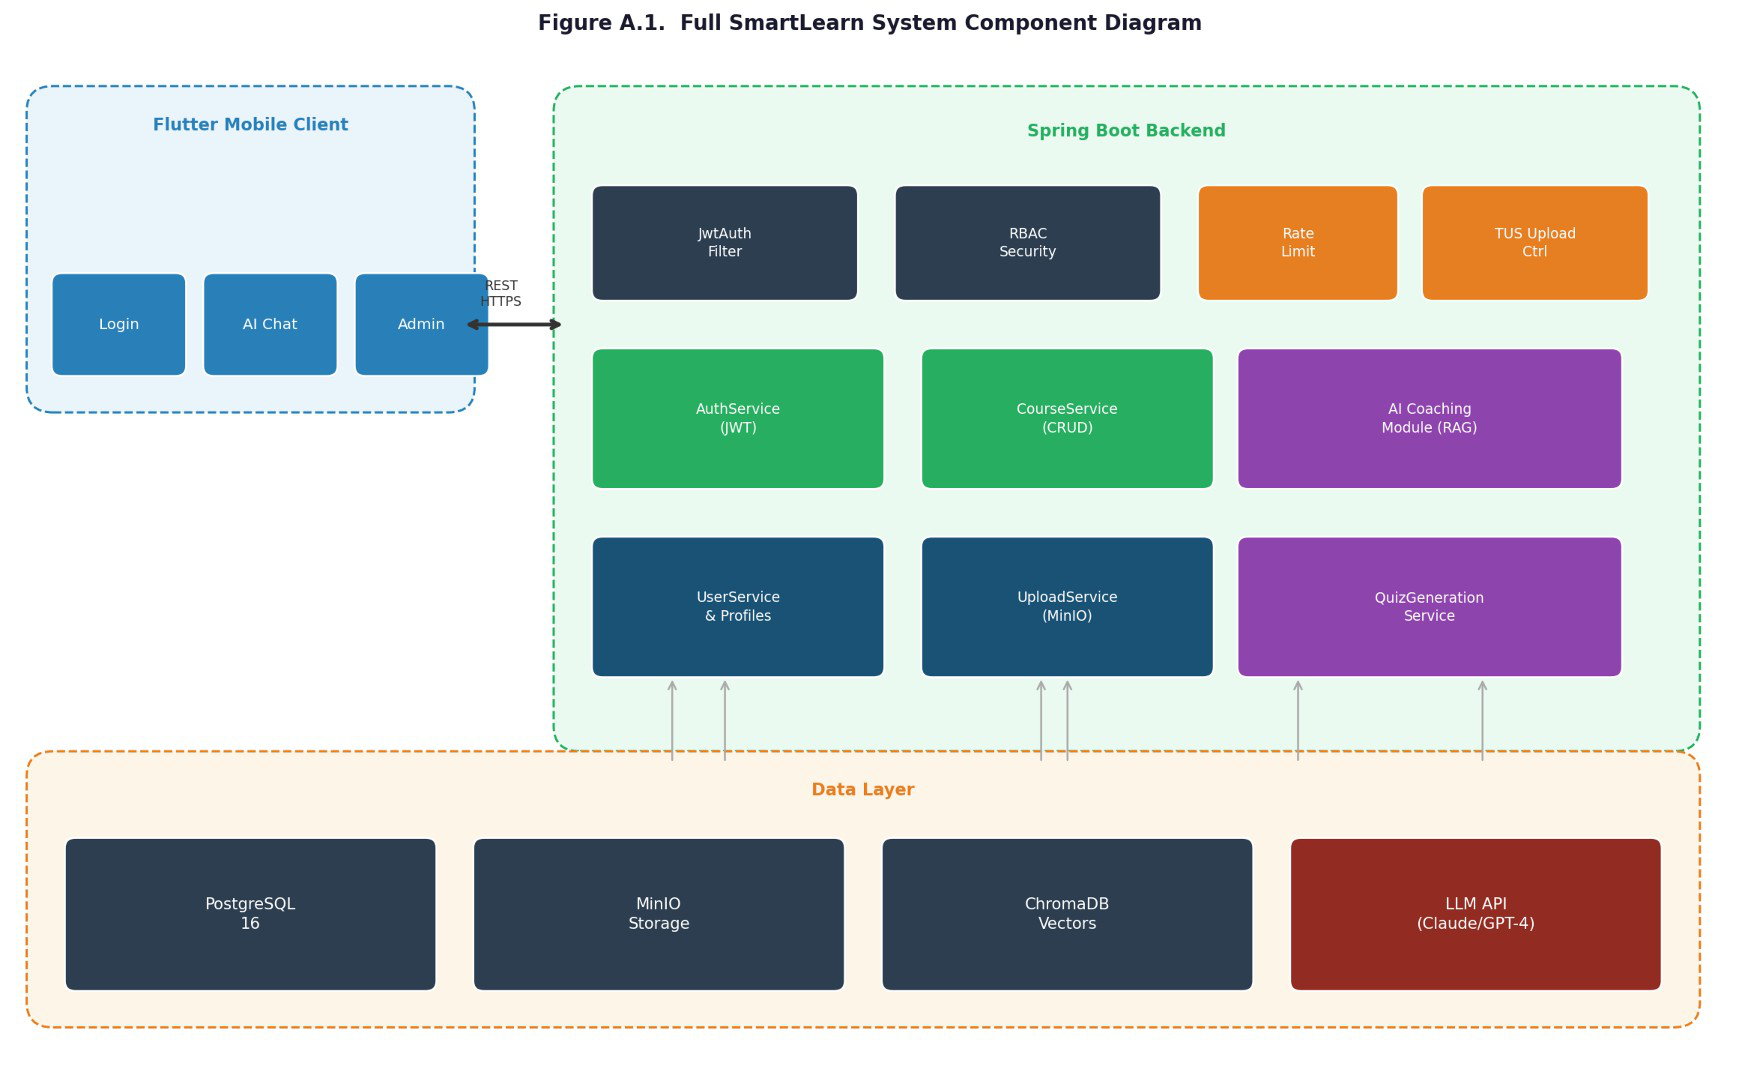
\includegraphics[width=\textwidth]{figs/figA_1_component.png}
\caption{Full SmartLearn system component diagram: Flutter client, Spring Boot backend
modules, PostgreSQL, MinIO, ChromaDB, and LLM API integration}
\label{fig:component}
\end{figure}

\begin{figure}[htbp]
\centering
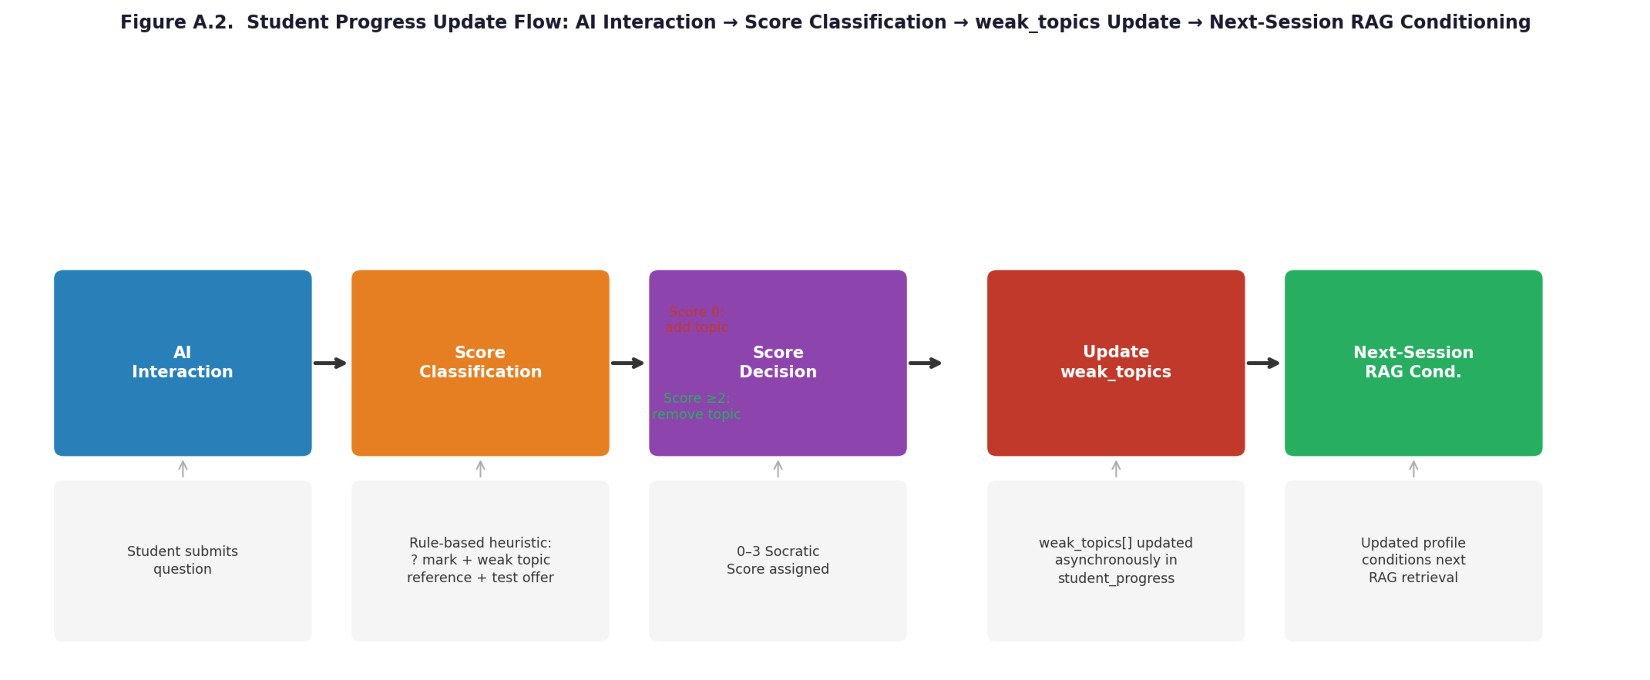
\includegraphics[width=\textwidth]{figs/figA_2_progress.png}
\caption{Student progress update flow: AI interaction \rar\ score classification \rar\
weak\_topics update \rar\ next-session RAG conditioning}
\label{fig:progressflow}
\end{figure}

\begin{figure}[htbp]
\centering
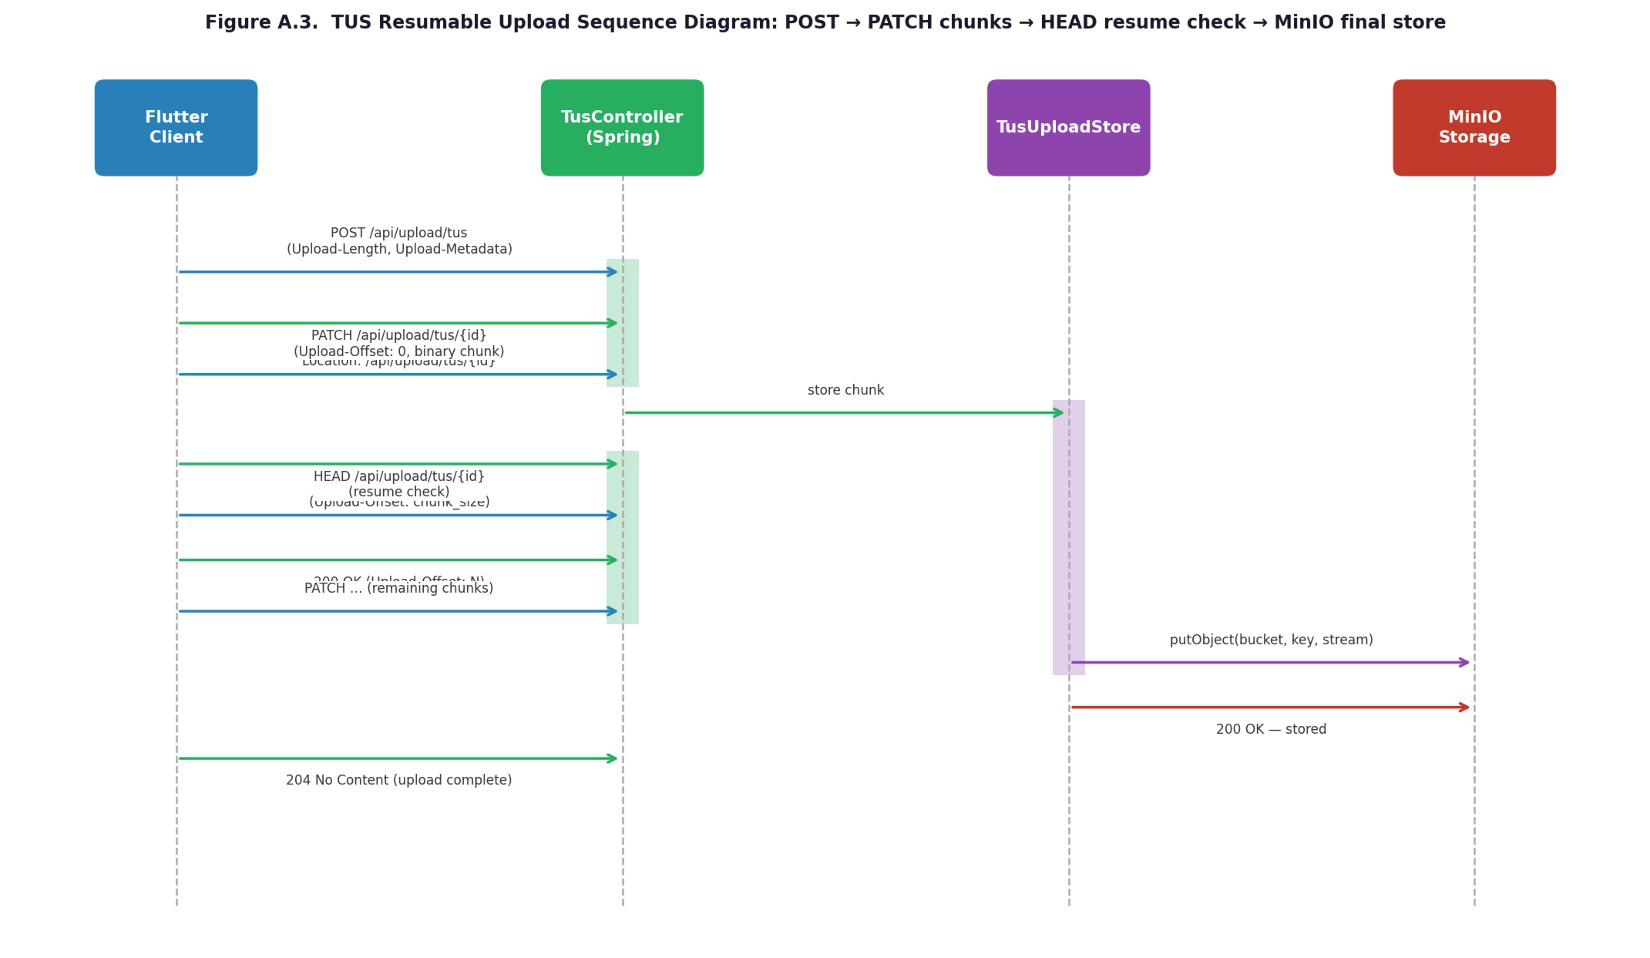
\includegraphics[width=0.92\textwidth]{figs/figA_3_tus.png}
\caption{TUS resumable upload sequence diagram: POST (create) \rar\ PATCH chunks \rar\ HEAD
(resume check) \rar\ MinIO final store}
\label{fig:tus}
\end{figure}

\chapter{REST API Endpoint Reference}
\addcontentsline{toc}{chapter}{Appendix B. REST API Endpoint Reference}

Table~\ref{tab:api} provides a complete reference of the SmartLearn REST API endpoints, their
HTTP methods, required roles, and descriptions.

\begin{longtable}{l L{4.6cm} L{2.6cm} L{4.0cm}}
\caption{SmartLearn REST API endpoint reference}\label{tab:api}\\
\toprule
\textbf{Method} & \textbf{Endpoint} & \textbf{Role Required} & \textbf{Description}\\
\midrule
\endfirsthead
\multicolumn{4}{l}{\small\itshape Table B.1 (continued)}\\
\toprule
\textbf{Method} & \textbf{Endpoint} & \textbf{Role Required} & \textbf{Description}\\
\midrule
\endhead
\bottomrule
\endfoot
POST & \texttt{/api/auth/register} & PUBLIC & Register new user\\
POST & \texttt{/api/auth/login} & PUBLIC & Authenticate and receive JWT\\
POST & \texttt{/api/auth/refresh} & PUBLIC & Refresh access token\\
GET & \texttt{/api/courses} & ALL & List all available courses\\
POST & \texttt{/api/courses} & TEACHER, ADMIN & Create new course\\
GET & \texttt{/api/courses/\{id\}} & ALL & Get course details and lessons\\
PUT & \texttt{/api/courses/\{id\}} & TEACHER, ADMIN & Update course metadata\\
DELETE & \texttt{/api/courses/\{id\}} & ADMIN & Delete course\\
POST & \texttt{/api/lessons} & TEACHER, ADMIN & Create lesson in a course\\
GET & \texttt{/api/progress/me} & STUDENT, ADMIN & Get own progress profile\\
PATCH & \texttt{/api/progress/\{id\}/weak-topics} & STUDENT, ADMIN & Update weak topics after
quiz\\
POST & \texttt{/api/ai/chat} & STUDENT, ADMIN & Send message to AI coach\\
GET & \texttt{/api/ai/history} & STUDENT, ADMIN & Retrieve AI chat history\\
POST & \texttt{/api/upload/tus} & TEACHER, ADMIN & Initiate TUS upload\\
GET & \texttt{/api/users} & ADMIN & List all users\\
PATCH & \texttt{/api/users/\{id\}/role} & ADMIN & Change user role\\
GET & \texttt{/api/badges/me} & STUDENT, ADMIN & Get earned badges\\
GET & \texttt{/api/leaderboard} & ALL & Get leaderboard rankings\\
\end{longtable}

%==============================================================================
%  AFFIRMATION
%==============================================================================
\chapter*{Affirmation}
\addcontentsline{toc}{chapter}{Affirmation}

I hereby affirm that this Bachelor Paper has been developed independently by me and that I
have not used any sources other than those listed in the References section. All citations
and references have been properly acknowledged. This work has not been previously submitted
for any academic degree.

\vspace{1.5cm}
\noindent Student: Azimjon Kurbanov \hfill Date: \rule{4cm}{0.4pt}

\end{document}
